% Created by tikzDevice version 0.12 on 2019-05-09 12:18:54
% !TEX encoding = UTF-8 Unicode
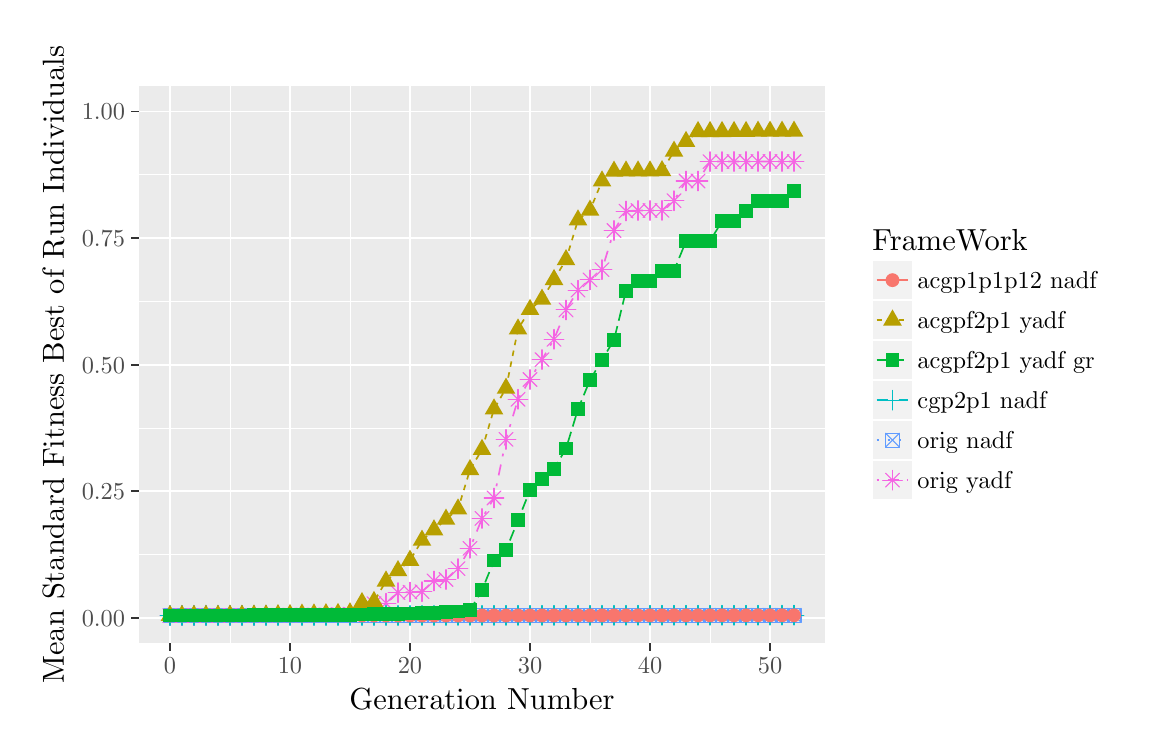
\begin{tikzpicture}[x=1pt,y=1pt]
\definecolor{fillColor}{RGB}{255,255,255}
\path[use as bounding box,fill=fillColor,fill opacity=0.00] (0,0) rectangle (397.48,252.94);
\begin{scope}
\path[clip] (  0.00,  0.00) rectangle (397.48,252.94);
\definecolor{drawColor}{RGB}{255,255,255}
\definecolor{fillColor}{RGB}{255,255,255}

\path[draw=drawColor,line width= 0.6pt,line join=round,line cap=round,fill=fillColor] (  0.00,  0.00) rectangle (397.48,252.95);
\end{scope}
\begin{scope}
\path[clip] ( 40.14, 30.56) rectangle (288.20,231.75);
\definecolor{fillColor}{gray}{0.92}

\path[fill=fillColor] ( 40.14, 30.56) rectangle (288.20,231.75);
\definecolor{drawColor}{RGB}{255,255,255}

\path[draw=drawColor,line width= 0.3pt,line join=round] ( 40.14, 62.57) --
	(288.20, 62.57);

\path[draw=drawColor,line width= 0.3pt,line join=round] ( 40.14,108.29) --
	(288.20,108.29);

\path[draw=drawColor,line width= 0.3pt,line join=round] ( 40.14,154.02) --
	(288.20,154.02);

\path[draw=drawColor,line width= 0.3pt,line join=round] ( 40.14,199.75) --
	(288.20,199.75);

\path[draw=drawColor,line width= 0.3pt,line join=round] ( 73.10, 30.56) --
	( 73.10,231.75);

\path[draw=drawColor,line width= 0.3pt,line join=round] (116.47, 30.56) --
	(116.47,231.75);

\path[draw=drawColor,line width= 0.3pt,line join=round] (159.83, 30.56) --
	(159.83,231.75);

\path[draw=drawColor,line width= 0.3pt,line join=round] (203.20, 30.56) --
	(203.20,231.75);

\path[draw=drawColor,line width= 0.3pt,line join=round] (246.57, 30.56) --
	(246.57,231.75);

\path[draw=drawColor,line width= 0.6pt,line join=round] ( 40.14, 39.70) --
	(288.20, 39.70);

\path[draw=drawColor,line width= 0.6pt,line join=round] ( 40.14, 85.43) --
	(288.20, 85.43);

\path[draw=drawColor,line width= 0.6pt,line join=round] ( 40.14,131.16) --
	(288.20,131.16);

\path[draw=drawColor,line width= 0.6pt,line join=round] ( 40.14,176.88) --
	(288.20,176.88);

\path[draw=drawColor,line width= 0.6pt,line join=round] ( 40.14,222.61) --
	(288.20,222.61);

\path[draw=drawColor,line width= 0.6pt,line join=round] ( 51.41, 30.56) --
	( 51.41,231.75);

\path[draw=drawColor,line width= 0.6pt,line join=round] ( 94.78, 30.56) --
	( 94.78,231.75);

\path[draw=drawColor,line width= 0.6pt,line join=round] (138.15, 30.56) --
	(138.15,231.75);

\path[draw=drawColor,line width= 0.6pt,line join=round] (181.52, 30.56) --
	(181.52,231.75);

\path[draw=drawColor,line width= 0.6pt,line join=round] (224.88, 30.56) --
	(224.88,231.75);

\path[draw=drawColor,line width= 0.6pt,line join=round] (268.25, 30.56) --
	(268.25,231.75);
\definecolor{drawColor}{RGB}{248,118,109}

\path[draw=drawColor,line width= 0.6pt,line join=round] ( 51.41, 40.49) --
	( 55.75, 40.50) --
	( 60.09, 40.51) --
	( 64.42, 40.51) --
	( 68.76, 40.51) --
	( 73.10, 40.51) --
	( 77.43, 40.51) --
	( 81.77, 40.51) --
	( 86.11, 40.51) --
	( 90.44, 40.51) --
	( 94.78, 40.51) --
	( 99.12, 40.51) --
	(103.45, 40.51) --
	(107.79, 40.51) --
	(112.13, 40.51) --
	(116.47, 40.52) --
	(120.80, 40.52) --
	(125.14, 40.52) --
	(129.48, 40.52) --
	(133.81, 40.52) --
	(138.15, 40.52) --
	(142.49, 40.52) --
	(146.82, 40.52) --
	(151.16, 40.52) --
	(155.50, 40.52) --
	(159.83, 40.52) --
	(164.17, 40.53) --
	(168.51, 40.53) --
	(172.84, 40.53) --
	(177.18, 40.54) --
	(181.52, 40.54) --
	(185.85, 40.55) --
	(190.19, 40.55) --
	(194.53, 40.55) --
	(198.86, 40.56) --
	(203.20, 40.56) --
	(207.54, 40.56) --
	(211.87, 40.56) --
	(216.21, 40.57) --
	(220.55, 40.57) --
	(224.88, 40.57) --
	(229.22, 40.57) --
	(233.56, 40.58) --
	(237.89, 40.58) --
	(242.23, 40.58) --
	(246.57, 40.59) --
	(250.90, 40.59) --
	(255.24, 40.59) --
	(259.58, 40.59) --
	(263.91, 40.60) --
	(268.25, 40.60) --
	(272.59, 40.60) --
	(276.92, 40.60);
\definecolor{drawColor}{RGB}{183,159,0}

\path[draw=drawColor,line width= 0.6pt,dash pattern=on 2pt off 2pt ,line join=round] ( 51.41, 40.51) --
	( 55.75, 40.53) --
	( 60.09, 40.55) --
	( 64.42, 40.56) --
	( 68.76, 40.58) --
	( 73.10, 40.59) --
	( 77.43, 40.62) --
	( 81.77, 40.65) --
	( 86.11, 40.68) --
	( 90.44, 40.78) --
	( 94.78, 40.81) --
	( 99.12, 40.99) --
	(103.45, 41.05) --
	(107.79, 41.12) --
	(112.13, 41.21) --
	(116.47, 41.47) --
	(120.80, 45.14) --
	(125.14, 45.57) --
	(129.48, 52.95) --
	(133.81, 56.69) --
	(138.15, 60.45) --
	(142.49, 67.68) --
	(146.82, 71.44) --
	(151.16, 75.28) --
	(155.50, 78.97) --
	(159.83, 93.18) --
	(164.17,100.49) --
	(168.51,115.13) --
	(172.84,122.60) --
	(177.18,144.01) --
	(181.52,151.07) --
	(185.85,154.76) --
	(190.19,161.89) --
	(194.53,169.05) --
	(198.86,183.43) --
	(203.20,186.95) --
	(207.54,197.50) --
	(211.87,201.03) --
	(216.21,201.10) --
	(220.55,201.11) --
	(224.88,201.11) --
	(229.22,201.21) --
	(233.56,208.25) --
	(237.89,211.78) --
	(242.23,215.37) --
	(246.57,215.38) --
	(250.90,215.38) --
	(255.24,215.39) --
	(259.58,215.39) --
	(263.91,215.48) --
	(268.25,215.48) --
	(272.59,215.48) --
	(276.92,215.48);
\definecolor{drawColor}{RGB}{0,186,56}

\path[draw=drawColor,line width= 0.6pt,dash pattern=on 4pt off 2pt ,line join=round] ( 51.41, 40.50) --
	( 55.75, 40.51) --
	( 60.09, 40.51) --
	( 64.42, 40.53) --
	( 68.76, 40.54) --
	( 73.10, 40.55) --
	( 77.43, 40.56) --
	( 81.77, 40.56) --
	( 86.11, 40.60) --
	( 90.44, 40.61) --
	( 94.78, 40.66) --
	( 99.12, 40.70) --
	(103.45, 40.71) --
	(107.79, 40.73) --
	(112.13, 40.79) --
	(116.47, 40.84) --
	(120.80, 40.89) --
	(125.14, 40.97) --
	(129.48, 41.09) --
	(133.81, 41.13) --
	(138.15, 41.27) --
	(142.49, 41.36) --
	(146.82, 41.56) --
	(151.16, 41.71) --
	(155.50, 41.99) --
	(159.83, 42.39) --
	(164.17, 49.69) --
	(168.51, 60.39) --
	(172.84, 64.16) --
	(177.18, 74.91) --
	(181.52, 85.78) --
	(185.85, 89.74) --
	(190.19, 93.48) --
	(194.53,100.85) --
	(198.86,115.08) --
	(203.20,125.63) --
	(207.54,132.89) --
	(211.87,140.09) --
	(216.21,157.91) --
	(220.55,161.45) --
	(224.88,161.47) --
	(229.22,165.03) --
	(233.56,165.15) --
	(237.89,175.77) --
	(242.23,175.79) --
	(246.57,175.88) --
	(250.90,183.00) --
	(255.24,183.15) --
	(259.58,186.74) --
	(263.91,190.33) --
	(268.25,190.33) --
	(272.59,190.33) --
	(276.92,193.91);
\definecolor{drawColor}{RGB}{0,191,196}

\path[draw=drawColor,line width= 0.6pt,dash pattern=on 4pt off 4pt ,line join=round] ( 51.41, 40.51) --
	( 55.75, 40.51) --
	( 60.09, 40.51) --
	( 64.42, 40.51) --
	( 68.76, 40.51) --
	( 73.10, 40.51) --
	( 77.43, 40.51) --
	( 81.77, 40.51) --
	( 86.11, 40.51) --
	( 90.44, 40.51) --
	( 94.78, 40.52) --
	( 99.12, 40.52) --
	(103.45, 40.52) --
	(107.79, 40.52) --
	(112.13, 40.53) --
	(116.47, 40.53) --
	(120.80, 40.53) --
	(125.14, 40.54) --
	(129.48, 40.54) --
	(133.81, 40.55) --
	(138.15, 40.55) --
	(142.49, 40.55) --
	(146.82, 40.55) --
	(151.16, 40.55) --
	(155.50, 40.56) --
	(159.83, 40.56) --
	(164.17, 40.56) --
	(168.51, 40.57) --
	(172.84, 40.57) --
	(177.18, 40.57) --
	(181.52, 40.57) --
	(185.85, 40.57) --
	(190.19, 40.57) --
	(194.53, 40.58) --
	(198.86, 40.58) --
	(203.20, 40.58) --
	(207.54, 40.59) --
	(211.87, 40.60) --
	(216.21, 40.60) --
	(220.55, 40.61) --
	(224.88, 40.61) --
	(229.22, 40.61) --
	(233.56, 40.62) --
	(237.89, 40.62) --
	(242.23, 40.63) --
	(246.57, 40.63) --
	(250.90, 40.63) --
	(255.24, 40.63) --
	(259.58, 40.64) --
	(263.91, 40.64) --
	(268.25, 40.64) --
	(272.59, 40.65) --
	(276.92, 40.66);
\definecolor{drawColor}{RGB}{97,156,255}

\path[draw=drawColor,line width= 0.6pt,dash pattern=on 1pt off 3pt ,line join=round] ( 51.41, 40.50) --
	( 55.75, 40.51) --
	( 60.09, 40.51) --
	( 64.42, 40.51) --
	( 68.76, 40.51) --
	( 73.10, 40.51) --
	( 77.43, 40.51) --
	( 81.77, 40.51) --
	( 86.11, 40.51) --
	( 90.44, 40.51) --
	( 94.78, 40.51) --
	( 99.12, 40.51) --
	(103.45, 40.51) --
	(107.79, 40.52) --
	(112.13, 40.52) --
	(116.47, 40.52) --
	(120.80, 40.52) --
	(125.14, 40.52) --
	(129.48, 40.52) --
	(133.81, 40.52) --
	(138.15, 40.52) --
	(142.49, 40.52) --
	(146.82, 40.52) --
	(151.16, 40.53) --
	(155.50, 40.53) --
	(159.83, 40.53) --
	(164.17, 40.53) --
	(168.51, 40.53) --
	(172.84, 40.54) --
	(177.18, 40.54) --
	(181.52, 40.54) --
	(185.85, 40.54) --
	(190.19, 40.54) --
	(194.53, 40.55) --
	(198.86, 40.56) --
	(203.20, 40.56) --
	(207.54, 40.56) --
	(211.87, 40.57) --
	(216.21, 40.57) --
	(220.55, 40.58) --
	(224.88, 40.58) --
	(229.22, 40.58) --
	(233.56, 40.58) --
	(237.89, 40.59) --
	(242.23, 40.59) --
	(246.57, 40.59) --
	(250.90, 40.60) --
	(255.24, 40.60) --
	(259.58, 40.61) --
	(263.91, 40.61) --
	(268.25, 40.61) --
	(272.59, 40.61) --
	(276.92, 40.61);
\definecolor{drawColor}{RGB}{245,100,227}

\path[draw=drawColor,line width= 0.6pt,dash pattern=on 1pt off 3pt on 4pt off 3pt ,line join=round] ( 51.41, 40.50) --
	( 55.75, 40.51) --
	( 60.09, 40.52) --
	( 64.42, 40.53) --
	( 68.76, 40.53) --
	( 73.10, 40.54) --
	( 77.43, 40.56) --
	( 81.77, 40.57) --
	( 86.11, 40.61) --
	( 90.44, 40.64) --
	( 94.78, 40.69) --
	( 99.12, 40.70) --
	(103.45, 40.74) --
	(107.79, 40.80) --
	(112.13, 40.90) --
	(116.47, 41.02) --
	(120.80, 41.15) --
	(125.14, 44.82) --
	(129.48, 44.97) --
	(133.81, 48.80) --
	(138.15, 49.00) --
	(142.49, 49.14) --
	(146.82, 53.01) --
	(151.16, 53.53) --
	(155.50, 57.48) --
	(159.83, 64.80) --
	(164.17, 75.60) --
	(168.51, 83.00) --
	(172.84,104.15) --
	(177.18,118.66) --
	(181.52,125.82) --
	(185.85,133.01) --
	(190.19,140.33) --
	(194.53,150.94) --
	(198.86,158.08) --
	(203.20,161.79) --
	(207.54,165.52) --
	(211.87,179.64) --
	(216.21,186.67) --
	(220.55,186.87) --
	(224.88,186.87) --
	(229.22,186.90) --
	(233.56,190.41) --
	(237.89,197.52) --
	(242.23,197.52) --
	(246.57,204.55) --
	(250.90,204.55) --
	(255.24,204.56) --
	(259.58,204.56) --
	(263.91,204.59) --
	(268.25,204.59) --
	(272.59,204.59) --
	(276.92,204.59);
\definecolor{drawColor}{RGB}{97,156,255}

\path[draw=drawColor,line width= 0.4pt,line join=round,line cap=round] ( 48.92, 38.00) rectangle ( 53.91, 42.99);

\path[draw=drawColor,line width= 0.4pt,line join=round,line cap=round] ( 48.92, 38.00) -- ( 53.91, 42.99);

\path[draw=drawColor,line width= 0.4pt,line join=round,line cap=round] ( 48.92, 42.99) -- ( 53.91, 38.00);

\path[draw=drawColor,line width= 0.4pt,line join=round,line cap=round] ( 53.25, 38.01) rectangle ( 58.25, 43.00);

\path[draw=drawColor,line width= 0.4pt,line join=round,line cap=round] ( 53.25, 38.01) -- ( 58.25, 43.00);

\path[draw=drawColor,line width= 0.4pt,line join=round,line cap=round] ( 53.25, 43.00) -- ( 58.25, 38.01);

\path[draw=drawColor,line width= 0.4pt,line join=round,line cap=round] ( 57.59, 38.01) rectangle ( 62.59, 43.01);

\path[draw=drawColor,line width= 0.4pt,line join=round,line cap=round] ( 57.59, 38.01) -- ( 62.59, 43.01);

\path[draw=drawColor,line width= 0.4pt,line join=round,line cap=round] ( 57.59, 43.01) -- ( 62.59, 38.01);

\path[draw=drawColor,line width= 0.4pt,line join=round,line cap=round] ( 61.93, 38.01) rectangle ( 66.92, 43.01);

\path[draw=drawColor,line width= 0.4pt,line join=round,line cap=round] ( 61.93, 38.01) -- ( 66.92, 43.01);

\path[draw=drawColor,line width= 0.4pt,line join=round,line cap=round] ( 61.93, 43.01) -- ( 66.92, 38.01);

\path[draw=drawColor,line width= 0.4pt,line join=round,line cap=round] ( 66.26, 38.01) rectangle ( 71.26, 43.01);

\path[draw=drawColor,line width= 0.4pt,line join=round,line cap=round] ( 66.26, 38.01) -- ( 71.26, 43.01);

\path[draw=drawColor,line width= 0.4pt,line join=round,line cap=round] ( 66.26, 43.01) -- ( 71.26, 38.01);

\path[draw=drawColor,line width= 0.4pt,line join=round,line cap=round] ( 70.60, 38.01) rectangle ( 75.60, 43.01);

\path[draw=drawColor,line width= 0.4pt,line join=round,line cap=round] ( 70.60, 38.01) -- ( 75.60, 43.01);

\path[draw=drawColor,line width= 0.4pt,line join=round,line cap=round] ( 70.60, 43.01) -- ( 75.60, 38.01);

\path[draw=drawColor,line width= 0.4pt,line join=round,line cap=round] ( 74.94, 38.01) rectangle ( 79.93, 43.01);

\path[draw=drawColor,line width= 0.4pt,line join=round,line cap=round] ( 74.94, 38.01) -- ( 79.93, 43.01);

\path[draw=drawColor,line width= 0.4pt,line join=round,line cap=round] ( 74.94, 43.01) -- ( 79.93, 38.01);

\path[draw=drawColor,line width= 0.4pt,line join=round,line cap=round] ( 79.27, 38.01) rectangle ( 84.27, 43.01);

\path[draw=drawColor,line width= 0.4pt,line join=round,line cap=round] ( 79.27, 38.01) -- ( 84.27, 43.01);

\path[draw=drawColor,line width= 0.4pt,line join=round,line cap=round] ( 79.27, 43.01) -- ( 84.27, 38.01);

\path[draw=drawColor,line width= 0.4pt,line join=round,line cap=round] ( 83.61, 38.01) rectangle ( 88.61, 43.01);

\path[draw=drawColor,line width= 0.4pt,line join=round,line cap=round] ( 83.61, 38.01) -- ( 88.61, 43.01);

\path[draw=drawColor,line width= 0.4pt,line join=round,line cap=round] ( 83.61, 43.01) -- ( 88.61, 38.01);

\path[draw=drawColor,line width= 0.4pt,line join=round,line cap=round] ( 87.95, 38.01) rectangle ( 92.94, 43.01);

\path[draw=drawColor,line width= 0.4pt,line join=round,line cap=round] ( 87.95, 38.01) -- ( 92.94, 43.01);

\path[draw=drawColor,line width= 0.4pt,line join=round,line cap=round] ( 87.95, 43.01) -- ( 92.94, 38.01);

\path[draw=drawColor,line width= 0.4pt,line join=round,line cap=round] ( 92.28, 38.02) rectangle ( 97.28, 43.01);

\path[draw=drawColor,line width= 0.4pt,line join=round,line cap=round] ( 92.28, 38.02) -- ( 97.28, 43.01);

\path[draw=drawColor,line width= 0.4pt,line join=round,line cap=round] ( 92.28, 43.01) -- ( 97.28, 38.02);

\path[draw=drawColor,line width= 0.4pt,line join=round,line cap=round] ( 96.62, 38.02) rectangle (101.62, 43.01);

\path[draw=drawColor,line width= 0.4pt,line join=round,line cap=round] ( 96.62, 38.02) -- (101.62, 43.01);

\path[draw=drawColor,line width= 0.4pt,line join=round,line cap=round] ( 96.62, 43.01) -- (101.62, 38.02);

\path[draw=drawColor,line width= 0.4pt,line join=round,line cap=round] (100.96, 38.02) rectangle (105.95, 43.01);

\path[draw=drawColor,line width= 0.4pt,line join=round,line cap=round] (100.96, 38.02) -- (105.95, 43.01);

\path[draw=drawColor,line width= 0.4pt,line join=round,line cap=round] (100.96, 43.01) -- (105.95, 38.02);

\path[draw=drawColor,line width= 0.4pt,line join=round,line cap=round] (105.29, 38.02) rectangle (110.29, 43.02);

\path[draw=drawColor,line width= 0.4pt,line join=round,line cap=round] (105.29, 38.02) -- (110.29, 43.02);

\path[draw=drawColor,line width= 0.4pt,line join=round,line cap=round] (105.29, 43.02) -- (110.29, 38.02);

\path[draw=drawColor,line width= 0.4pt,line join=round,line cap=round] (109.63, 38.02) rectangle (114.63, 43.02);

\path[draw=drawColor,line width= 0.4pt,line join=round,line cap=round] (109.63, 38.02) -- (114.63, 43.02);

\path[draw=drawColor,line width= 0.4pt,line join=round,line cap=round] (109.63, 43.02) -- (114.63, 38.02);

\path[draw=drawColor,line width= 0.4pt,line join=round,line cap=round] (113.97, 38.02) rectangle (118.96, 43.02);

\path[draw=drawColor,line width= 0.4pt,line join=round,line cap=round] (113.97, 38.02) -- (118.96, 43.02);

\path[draw=drawColor,line width= 0.4pt,line join=round,line cap=round] (113.97, 43.02) -- (118.96, 38.02);

\path[draw=drawColor,line width= 0.4pt,line join=round,line cap=round] (118.30, 38.02) rectangle (123.30, 43.02);

\path[draw=drawColor,line width= 0.4pt,line join=round,line cap=round] (118.30, 38.02) -- (123.30, 43.02);

\path[draw=drawColor,line width= 0.4pt,line join=round,line cap=round] (118.30, 43.02) -- (123.30, 38.02);

\path[draw=drawColor,line width= 0.4pt,line join=round,line cap=round] (122.64, 38.02) rectangle (127.64, 43.02);

\path[draw=drawColor,line width= 0.4pt,line join=round,line cap=round] (122.64, 38.02) -- (127.64, 43.02);

\path[draw=drawColor,line width= 0.4pt,line join=round,line cap=round] (122.64, 43.02) -- (127.64, 38.02);

\path[draw=drawColor,line width= 0.4pt,line join=round,line cap=round] (126.98, 38.02) rectangle (131.97, 43.02);

\path[draw=drawColor,line width= 0.4pt,line join=round,line cap=round] (126.98, 38.02) -- (131.97, 43.02);

\path[draw=drawColor,line width= 0.4pt,line join=round,line cap=round] (126.98, 43.02) -- (131.97, 38.02);

\path[draw=drawColor,line width= 0.4pt,line join=round,line cap=round] (131.31, 38.02) rectangle (136.31, 43.02);

\path[draw=drawColor,line width= 0.4pt,line join=round,line cap=round] (131.31, 38.02) -- (136.31, 43.02);

\path[draw=drawColor,line width= 0.4pt,line join=round,line cap=round] (131.31, 43.02) -- (136.31, 38.02);

\path[draw=drawColor,line width= 0.4pt,line join=round,line cap=round] (135.65, 38.02) rectangle (140.65, 43.02);

\path[draw=drawColor,line width= 0.4pt,line join=round,line cap=round] (135.65, 38.02) -- (140.65, 43.02);

\path[draw=drawColor,line width= 0.4pt,line join=round,line cap=round] (135.65, 43.02) -- (140.65, 38.02);

\path[draw=drawColor,line width= 0.4pt,line join=round,line cap=round] (139.99, 38.02) rectangle (144.98, 43.02);

\path[draw=drawColor,line width= 0.4pt,line join=round,line cap=round] (139.99, 38.02) -- (144.98, 43.02);

\path[draw=drawColor,line width= 0.4pt,line join=round,line cap=round] (139.99, 43.02) -- (144.98, 38.02);

\path[draw=drawColor,line width= 0.4pt,line join=round,line cap=round] (144.32, 38.02) rectangle (149.32, 43.02);

\path[draw=drawColor,line width= 0.4pt,line join=round,line cap=round] (144.32, 38.02) -- (149.32, 43.02);

\path[draw=drawColor,line width= 0.4pt,line join=round,line cap=round] (144.32, 43.02) -- (149.32, 38.02);

\path[draw=drawColor,line width= 0.4pt,line join=round,line cap=round] (148.66, 38.03) rectangle (153.66, 43.02);

\path[draw=drawColor,line width= 0.4pt,line join=round,line cap=round] (148.66, 38.03) -- (153.66, 43.02);

\path[draw=drawColor,line width= 0.4pt,line join=round,line cap=round] (148.66, 43.02) -- (153.66, 38.03);

\path[draw=drawColor,line width= 0.4pt,line join=round,line cap=round] (153.00, 38.03) rectangle (157.99, 43.03);

\path[draw=drawColor,line width= 0.4pt,line join=round,line cap=round] (153.00, 38.03) -- (157.99, 43.03);

\path[draw=drawColor,line width= 0.4pt,line join=round,line cap=round] (153.00, 43.03) -- (157.99, 38.03);

\path[draw=drawColor,line width= 0.4pt,line join=round,line cap=round] (157.33, 38.04) rectangle (162.33, 43.03);

\path[draw=drawColor,line width= 0.4pt,line join=round,line cap=round] (157.33, 38.04) -- (162.33, 43.03);

\path[draw=drawColor,line width= 0.4pt,line join=round,line cap=round] (157.33, 43.03) -- (162.33, 38.04);

\path[draw=drawColor,line width= 0.4pt,line join=round,line cap=round] (161.67, 38.04) rectangle (166.67, 43.03);

\path[draw=drawColor,line width= 0.4pt,line join=round,line cap=round] (161.67, 38.04) -- (166.67, 43.03);

\path[draw=drawColor,line width= 0.4pt,line join=round,line cap=round] (161.67, 43.03) -- (166.67, 38.04);

\path[draw=drawColor,line width= 0.4pt,line join=round,line cap=round] (166.01, 38.04) rectangle (171.00, 43.03);

\path[draw=drawColor,line width= 0.4pt,line join=round,line cap=round] (166.01, 38.04) -- (171.00, 43.03);

\path[draw=drawColor,line width= 0.4pt,line join=round,line cap=round] (166.01, 43.03) -- (171.00, 38.04);

\path[draw=drawColor,line width= 0.4pt,line join=round,line cap=round] (170.35, 38.04) rectangle (175.34, 43.03);

\path[draw=drawColor,line width= 0.4pt,line join=round,line cap=round] (170.35, 38.04) -- (175.34, 43.03);

\path[draw=drawColor,line width= 0.4pt,line join=round,line cap=round] (170.35, 43.03) -- (175.34, 38.04);

\path[draw=drawColor,line width= 0.4pt,line join=round,line cap=round] (174.68, 38.04) rectangle (179.68, 43.03);

\path[draw=drawColor,line width= 0.4pt,line join=round,line cap=round] (174.68, 38.04) -- (179.68, 43.03);

\path[draw=drawColor,line width= 0.4pt,line join=round,line cap=round] (174.68, 43.03) -- (179.68, 38.04);

\path[draw=drawColor,line width= 0.4pt,line join=round,line cap=round] (179.02, 38.04) rectangle (184.01, 43.04);

\path[draw=drawColor,line width= 0.4pt,line join=round,line cap=round] (179.02, 38.04) -- (184.01, 43.04);

\path[draw=drawColor,line width= 0.4pt,line join=round,line cap=round] (179.02, 43.04) -- (184.01, 38.04);

\path[draw=drawColor,line width= 0.4pt,line join=round,line cap=round] (183.36, 38.04) rectangle (188.35, 43.04);

\path[draw=drawColor,line width= 0.4pt,line join=round,line cap=round] (183.36, 38.04) -- (188.35, 43.04);

\path[draw=drawColor,line width= 0.4pt,line join=round,line cap=round] (183.36, 43.04) -- (188.35, 38.04);

\path[draw=drawColor,line width= 0.4pt,line join=round,line cap=round] (187.69, 38.05) rectangle (192.69, 43.04);

\path[draw=drawColor,line width= 0.4pt,line join=round,line cap=round] (187.69, 38.05) -- (192.69, 43.04);

\path[draw=drawColor,line width= 0.4pt,line join=round,line cap=round] (187.69, 43.04) -- (192.69, 38.05);

\path[draw=drawColor,line width= 0.4pt,line join=round,line cap=round] (192.03, 38.05) rectangle (197.02, 43.05);

\path[draw=drawColor,line width= 0.4pt,line join=round,line cap=round] (192.03, 38.05) -- (197.02, 43.05);

\path[draw=drawColor,line width= 0.4pt,line join=round,line cap=round] (192.03, 43.05) -- (197.02, 38.05);

\path[draw=drawColor,line width= 0.4pt,line join=round,line cap=round] (196.37, 38.06) rectangle (201.36, 43.06);

\path[draw=drawColor,line width= 0.4pt,line join=round,line cap=round] (196.37, 38.06) -- (201.36, 43.06);

\path[draw=drawColor,line width= 0.4pt,line join=round,line cap=round] (196.37, 43.06) -- (201.36, 38.06);

\path[draw=drawColor,line width= 0.4pt,line join=round,line cap=round] (200.70, 38.06) rectangle (205.70, 43.06);

\path[draw=drawColor,line width= 0.4pt,line join=round,line cap=round] (200.70, 38.06) -- (205.70, 43.06);

\path[draw=drawColor,line width= 0.4pt,line join=round,line cap=round] (200.70, 43.06) -- (205.70, 38.06);

\path[draw=drawColor,line width= 0.4pt,line join=round,line cap=round] (205.04, 38.07) rectangle (210.03, 43.06);

\path[draw=drawColor,line width= 0.4pt,line join=round,line cap=round] (205.04, 38.07) -- (210.03, 43.06);

\path[draw=drawColor,line width= 0.4pt,line join=round,line cap=round] (205.04, 43.06) -- (210.03, 38.07);

\path[draw=drawColor,line width= 0.4pt,line join=round,line cap=round] (209.38, 38.07) rectangle (214.37, 43.07);

\path[draw=drawColor,line width= 0.4pt,line join=round,line cap=round] (209.38, 38.07) -- (214.37, 43.07);

\path[draw=drawColor,line width= 0.4pt,line join=round,line cap=round] (209.38, 43.07) -- (214.37, 38.07);

\path[draw=drawColor,line width= 0.4pt,line join=round,line cap=round] (213.71, 38.07) rectangle (218.71, 43.07);

\path[draw=drawColor,line width= 0.4pt,line join=round,line cap=round] (213.71, 38.07) -- (218.71, 43.07);

\path[draw=drawColor,line width= 0.4pt,line join=round,line cap=round] (213.71, 43.07) -- (218.71, 38.07);

\path[draw=drawColor,line width= 0.4pt,line join=round,line cap=round] (218.05, 38.08) rectangle (223.04, 43.07);

\path[draw=drawColor,line width= 0.4pt,line join=round,line cap=round] (218.05, 38.08) -- (223.04, 43.07);

\path[draw=drawColor,line width= 0.4pt,line join=round,line cap=round] (218.05, 43.07) -- (223.04, 38.08);

\path[draw=drawColor,line width= 0.4pt,line join=round,line cap=round] (222.39, 38.08) rectangle (227.38, 43.07);

\path[draw=drawColor,line width= 0.4pt,line join=round,line cap=round] (222.39, 38.08) -- (227.38, 43.07);

\path[draw=drawColor,line width= 0.4pt,line join=round,line cap=round] (222.39, 43.07) -- (227.38, 38.08);

\path[draw=drawColor,line width= 0.4pt,line join=round,line cap=round] (226.72, 38.08) rectangle (231.72, 43.07);

\path[draw=drawColor,line width= 0.4pt,line join=round,line cap=round] (226.72, 38.08) -- (231.72, 43.07);

\path[draw=drawColor,line width= 0.4pt,line join=round,line cap=round] (226.72, 43.07) -- (231.72, 38.08);

\path[draw=drawColor,line width= 0.4pt,line join=round,line cap=round] (231.06, 38.08) rectangle (236.05, 43.08);

\path[draw=drawColor,line width= 0.4pt,line join=round,line cap=round] (231.06, 38.08) -- (236.05, 43.08);

\path[draw=drawColor,line width= 0.4pt,line join=round,line cap=round] (231.06, 43.08) -- (236.05, 38.08);

\path[draw=drawColor,line width= 0.4pt,line join=round,line cap=round] (235.40, 38.09) rectangle (240.39, 43.09);

\path[draw=drawColor,line width= 0.4pt,line join=round,line cap=round] (235.40, 38.09) -- (240.39, 43.09);

\path[draw=drawColor,line width= 0.4pt,line join=round,line cap=round] (235.40, 43.09) -- (240.39, 38.09);

\path[draw=drawColor,line width= 0.4pt,line join=round,line cap=round] (239.73, 38.09) rectangle (244.73, 43.09);

\path[draw=drawColor,line width= 0.4pt,line join=round,line cap=round] (239.73, 38.09) -- (244.73, 43.09);

\path[draw=drawColor,line width= 0.4pt,line join=round,line cap=round] (239.73, 43.09) -- (244.73, 38.09);

\path[draw=drawColor,line width= 0.4pt,line join=round,line cap=round] (244.07, 38.10) rectangle (249.06, 43.09);

\path[draw=drawColor,line width= 0.4pt,line join=round,line cap=round] (244.07, 38.10) -- (249.06, 43.09);

\path[draw=drawColor,line width= 0.4pt,line join=round,line cap=round] (244.07, 43.09) -- (249.06, 38.10);

\path[draw=drawColor,line width= 0.4pt,line join=round,line cap=round] (248.41, 38.10) rectangle (253.40, 43.10);

\path[draw=drawColor,line width= 0.4pt,line join=round,line cap=round] (248.41, 38.10) -- (253.40, 43.10);

\path[draw=drawColor,line width= 0.4pt,line join=round,line cap=round] (248.41, 43.10) -- (253.40, 38.10);

\path[draw=drawColor,line width= 0.4pt,line join=round,line cap=round] (252.74, 38.10) rectangle (257.74, 43.10);

\path[draw=drawColor,line width= 0.4pt,line join=round,line cap=round] (252.74, 38.10) -- (257.74, 43.10);

\path[draw=drawColor,line width= 0.4pt,line join=round,line cap=round] (252.74, 43.10) -- (257.74, 38.10);

\path[draw=drawColor,line width= 0.4pt,line join=round,line cap=round] (257.08, 38.11) rectangle (262.07, 43.10);

\path[draw=drawColor,line width= 0.4pt,line join=round,line cap=round] (257.08, 38.11) -- (262.07, 43.10);

\path[draw=drawColor,line width= 0.4pt,line join=round,line cap=round] (257.08, 43.10) -- (262.07, 38.11);

\path[draw=drawColor,line width= 0.4pt,line join=round,line cap=round] (261.42, 38.11) rectangle (266.41, 43.11);

\path[draw=drawColor,line width= 0.4pt,line join=round,line cap=round] (261.42, 38.11) -- (266.41, 43.11);

\path[draw=drawColor,line width= 0.4pt,line join=round,line cap=round] (261.42, 43.11) -- (266.41, 38.11);

\path[draw=drawColor,line width= 0.4pt,line join=round,line cap=round] (265.75, 38.11) rectangle (270.75, 43.11);

\path[draw=drawColor,line width= 0.4pt,line join=round,line cap=round] (265.75, 38.11) -- (270.75, 43.11);

\path[draw=drawColor,line width= 0.4pt,line join=round,line cap=round] (265.75, 43.11) -- (270.75, 38.11);

\path[draw=drawColor,line width= 0.4pt,line join=round,line cap=round] (270.09, 38.12) rectangle (275.09, 43.11);

\path[draw=drawColor,line width= 0.4pt,line join=round,line cap=round] (270.09, 38.12) -- (275.09, 43.11);

\path[draw=drawColor,line width= 0.4pt,line join=round,line cap=round] (270.09, 43.11) -- (275.09, 38.12);

\path[draw=drawColor,line width= 0.4pt,line join=round,line cap=round] (274.43, 38.12) rectangle (279.42, 43.11);

\path[draw=drawColor,line width= 0.4pt,line join=round,line cap=round] (274.43, 38.12) -- (279.42, 43.11);

\path[draw=drawColor,line width= 0.4pt,line join=round,line cap=round] (274.43, 43.11) -- (279.42, 38.12);
\definecolor{drawColor}{RGB}{245,100,227}

\path[draw=drawColor,line width= 0.4pt,line join=round,line cap=round] ( 48.92, 38.00) -- ( 53.91, 43.00);

\path[draw=drawColor,line width= 0.4pt,line join=round,line cap=round] ( 48.92, 43.00) -- ( 53.91, 38.00);

\path[draw=drawColor,line width= 0.4pt,line join=round,line cap=round] ( 47.88, 40.50) -- ( 54.95, 40.50);

\path[draw=drawColor,line width= 0.4pt,line join=round,line cap=round] ( 51.41, 36.97) -- ( 51.41, 44.03);

\path[draw=drawColor,line width= 0.4pt,line join=round,line cap=round] ( 53.25, 38.01) -- ( 58.25, 43.01);

\path[draw=drawColor,line width= 0.4pt,line join=round,line cap=round] ( 53.25, 43.01) -- ( 58.25, 38.01);

\path[draw=drawColor,line width= 0.4pt,line join=round,line cap=round] ( 52.22, 40.51) -- ( 59.28, 40.51);

\path[draw=drawColor,line width= 0.4pt,line join=round,line cap=round] ( 55.75, 36.98) -- ( 55.75, 44.04);

\path[draw=drawColor,line width= 0.4pt,line join=round,line cap=round] ( 57.59, 38.02) -- ( 62.59, 43.02);

\path[draw=drawColor,line width= 0.4pt,line join=round,line cap=round] ( 57.59, 43.02) -- ( 62.59, 38.02);

\path[draw=drawColor,line width= 0.4pt,line join=round,line cap=round] ( 56.56, 40.52) -- ( 63.62, 40.52);

\path[draw=drawColor,line width= 0.4pt,line join=round,line cap=round] ( 60.09, 36.99) -- ( 60.09, 44.05);

\path[draw=drawColor,line width= 0.4pt,line join=round,line cap=round] ( 61.93, 38.03) -- ( 66.92, 43.02);

\path[draw=drawColor,line width= 0.4pt,line join=round,line cap=round] ( 61.93, 43.02) -- ( 66.92, 38.03);

\path[draw=drawColor,line width= 0.4pt,line join=round,line cap=round] ( 60.89, 40.53) -- ( 67.96, 40.53);

\path[draw=drawColor,line width= 0.4pt,line join=round,line cap=round] ( 64.42, 36.99) -- ( 64.42, 44.06);

\path[draw=drawColor,line width= 0.4pt,line join=round,line cap=round] ( 66.26, 38.03) -- ( 71.26, 43.03);

\path[draw=drawColor,line width= 0.4pt,line join=round,line cap=round] ( 66.26, 43.03) -- ( 71.26, 38.03);

\path[draw=drawColor,line width= 0.4pt,line join=round,line cap=round] ( 65.23, 40.53) -- ( 72.29, 40.53);

\path[draw=drawColor,line width= 0.4pt,line join=round,line cap=round] ( 68.76, 37.00) -- ( 68.76, 44.06);

\path[draw=drawColor,line width= 0.4pt,line join=round,line cap=round] ( 70.60, 38.05) -- ( 75.60, 43.04);

\path[draw=drawColor,line width= 0.4pt,line join=round,line cap=round] ( 70.60, 43.04) -- ( 75.60, 38.05);

\path[draw=drawColor,line width= 0.4pt,line join=round,line cap=round] ( 69.57, 40.54) -- ( 76.63, 40.54);

\path[draw=drawColor,line width= 0.4pt,line join=round,line cap=round] ( 73.10, 37.01) -- ( 73.10, 44.08);

\path[draw=drawColor,line width= 0.4pt,line join=round,line cap=round] ( 74.94, 38.06) -- ( 79.93, 43.05);

\path[draw=drawColor,line width= 0.4pt,line join=round,line cap=round] ( 74.94, 43.05) -- ( 79.93, 38.06);

\path[draw=drawColor,line width= 0.4pt,line join=round,line cap=round] ( 73.90, 40.56) -- ( 80.97, 40.56);

\path[draw=drawColor,line width= 0.4pt,line join=round,line cap=round] ( 77.43, 37.02) -- ( 77.43, 44.09);

\path[draw=drawColor,line width= 0.4pt,line join=round,line cap=round] ( 79.27, 38.07) -- ( 84.27, 43.07);

\path[draw=drawColor,line width= 0.4pt,line join=round,line cap=round] ( 79.27, 43.07) -- ( 84.27, 38.07);

\path[draw=drawColor,line width= 0.4pt,line join=round,line cap=round] ( 78.24, 40.57) -- ( 85.30, 40.57);

\path[draw=drawColor,line width= 0.4pt,line join=round,line cap=round] ( 81.77, 37.04) -- ( 81.77, 44.10);

\path[draw=drawColor,line width= 0.4pt,line join=round,line cap=round] ( 83.61, 38.11) -- ( 88.61, 43.11);

\path[draw=drawColor,line width= 0.4pt,line join=round,line cap=round] ( 83.61, 43.11) -- ( 88.61, 38.11);

\path[draw=drawColor,line width= 0.4pt,line join=round,line cap=round] ( 82.58, 40.61) -- ( 89.64, 40.61);

\path[draw=drawColor,line width= 0.4pt,line join=round,line cap=round] ( 86.11, 37.08) -- ( 86.11, 44.14);

\path[draw=drawColor,line width= 0.4pt,line join=round,line cap=round] ( 87.95, 38.14) -- ( 92.94, 43.14);

\path[draw=drawColor,line width= 0.4pt,line join=round,line cap=round] ( 87.95, 43.14) -- ( 92.94, 38.14);

\path[draw=drawColor,line width= 0.4pt,line join=round,line cap=round] ( 86.91, 40.64) -- ( 93.98, 40.64);

\path[draw=drawColor,line width= 0.4pt,line join=round,line cap=round] ( 90.44, 37.11) -- ( 90.44, 44.17);

\path[draw=drawColor,line width= 0.4pt,line join=round,line cap=round] ( 92.28, 38.20) -- ( 97.28, 43.19);

\path[draw=drawColor,line width= 0.4pt,line join=round,line cap=round] ( 92.28, 43.19) -- ( 97.28, 38.20);

\path[draw=drawColor,line width= 0.4pt,line join=round,line cap=round] ( 91.25, 40.69) -- ( 98.31, 40.69);

\path[draw=drawColor,line width= 0.4pt,line join=round,line cap=round] ( 94.78, 37.16) -- ( 94.78, 44.23);

\path[draw=drawColor,line width= 0.4pt,line join=round,line cap=round] ( 96.62, 38.20) -- (101.62, 43.20);

\path[draw=drawColor,line width= 0.4pt,line join=round,line cap=round] ( 96.62, 43.20) -- (101.62, 38.20);

\path[draw=drawColor,line width= 0.4pt,line join=round,line cap=round] ( 95.59, 40.70) -- (102.65, 40.70);

\path[draw=drawColor,line width= 0.4pt,line join=round,line cap=round] ( 99.12, 37.17) -- ( 99.12, 44.23);

\path[draw=drawColor,line width= 0.4pt,line join=round,line cap=round] (100.96, 38.24) -- (105.95, 43.24);

\path[draw=drawColor,line width= 0.4pt,line join=round,line cap=round] (100.96, 43.24) -- (105.95, 38.24);

\path[draw=drawColor,line width= 0.4pt,line join=round,line cap=round] ( 99.92, 40.74) -- (106.99, 40.74);

\path[draw=drawColor,line width= 0.4pt,line join=round,line cap=round] (103.45, 37.21) -- (103.45, 44.27);

\path[draw=drawColor,line width= 0.4pt,line join=round,line cap=round] (105.29, 38.30) -- (110.29, 43.29);

\path[draw=drawColor,line width= 0.4pt,line join=round,line cap=round] (105.29, 43.29) -- (110.29, 38.30);

\path[draw=drawColor,line width= 0.4pt,line join=round,line cap=round] (104.26, 40.80) -- (111.32, 40.80);

\path[draw=drawColor,line width= 0.4pt,line join=round,line cap=round] (107.79, 37.26) -- (107.79, 44.33);

\path[draw=drawColor,line width= 0.4pt,line join=round,line cap=round] (109.63, 38.40) -- (114.63, 43.40);

\path[draw=drawColor,line width= 0.4pt,line join=round,line cap=round] (109.63, 43.40) -- (114.63, 38.40);

\path[draw=drawColor,line width= 0.4pt,line join=round,line cap=round] (108.60, 40.90) -- (115.66, 40.90);

\path[draw=drawColor,line width= 0.4pt,line join=round,line cap=round] (112.13, 37.37) -- (112.13, 44.43);

\path[draw=drawColor,line width= 0.4pt,line join=round,line cap=round] (113.97, 38.52) -- (118.96, 43.52);

\path[draw=drawColor,line width= 0.4pt,line join=round,line cap=round] (113.97, 43.52) -- (118.96, 38.52);

\path[draw=drawColor,line width= 0.4pt,line join=round,line cap=round] (112.93, 41.02) -- (120.00, 41.02);

\path[draw=drawColor,line width= 0.4pt,line join=round,line cap=round] (116.47, 37.49) -- (116.47, 44.55);

\path[draw=drawColor,line width= 0.4pt,line join=round,line cap=round] (118.30, 38.65) -- (123.30, 43.65);

\path[draw=drawColor,line width= 0.4pt,line join=round,line cap=round] (118.30, 43.65) -- (123.30, 38.65);

\path[draw=drawColor,line width= 0.4pt,line join=round,line cap=round] (117.27, 41.15) -- (124.33, 41.15);

\path[draw=drawColor,line width= 0.4pt,line join=round,line cap=round] (120.80, 37.62) -- (120.80, 44.68);

\path[draw=drawColor,line width= 0.4pt,line join=round,line cap=round] (122.64, 42.32) -- (127.64, 47.32);

\path[draw=drawColor,line width= 0.4pt,line join=round,line cap=round] (122.64, 47.32) -- (127.64, 42.32);

\path[draw=drawColor,line width= 0.4pt,line join=round,line cap=round] (121.61, 44.82) -- (128.67, 44.82);

\path[draw=drawColor,line width= 0.4pt,line join=round,line cap=round] (125.14, 41.29) -- (125.14, 48.35);

\path[draw=drawColor,line width= 0.4pt,line join=round,line cap=round] (126.98, 42.47) -- (131.97, 47.47);

\path[draw=drawColor,line width= 0.4pt,line join=round,line cap=round] (126.98, 47.47) -- (131.97, 42.47);

\path[draw=drawColor,line width= 0.4pt,line join=round,line cap=round] (125.94, 44.97) -- (133.01, 44.97);

\path[draw=drawColor,line width= 0.4pt,line join=round,line cap=round] (129.48, 41.44) -- (129.48, 48.50);

\path[draw=drawColor,line width= 0.4pt,line join=round,line cap=round] (131.31, 46.30) -- (136.31, 51.29);

\path[draw=drawColor,line width= 0.4pt,line join=round,line cap=round] (131.31, 51.29) -- (136.31, 46.30);

\path[draw=drawColor,line width= 0.4pt,line join=round,line cap=round] (130.28, 48.80) -- (137.34, 48.80);

\path[draw=drawColor,line width= 0.4pt,line join=round,line cap=round] (133.81, 45.26) -- (133.81, 52.33);

\path[draw=drawColor,line width= 0.4pt,line join=round,line cap=round] (135.65, 46.50) -- (140.65, 51.49);

\path[draw=drawColor,line width= 0.4pt,line join=round,line cap=round] (135.65, 51.49) -- (140.65, 46.50);

\path[draw=drawColor,line width= 0.4pt,line join=round,line cap=round] (134.62, 49.00) -- (141.68, 49.00);

\path[draw=drawColor,line width= 0.4pt,line join=round,line cap=round] (138.15, 45.47) -- (138.15, 52.53);

\path[draw=drawColor,line width= 0.4pt,line join=round,line cap=round] (139.99, 46.64) -- (144.98, 51.64);

\path[draw=drawColor,line width= 0.4pt,line join=round,line cap=round] (139.99, 51.64) -- (144.98, 46.64);

\path[draw=drawColor,line width= 0.4pt,line join=round,line cap=round] (138.95, 49.14) -- (146.02, 49.14);

\path[draw=drawColor,line width= 0.4pt,line join=round,line cap=round] (142.49, 45.61) -- (142.49, 52.67);

\path[draw=drawColor,line width= 0.4pt,line join=round,line cap=round] (144.32, 50.52) -- (149.32, 55.51);

\path[draw=drawColor,line width= 0.4pt,line join=round,line cap=round] (144.32, 55.51) -- (149.32, 50.52);

\path[draw=drawColor,line width= 0.4pt,line join=round,line cap=round] (143.29, 53.01) -- (150.35, 53.01);

\path[draw=drawColor,line width= 0.4pt,line join=round,line cap=round] (146.82, 49.48) -- (146.82, 56.54);

\path[draw=drawColor,line width= 0.4pt,line join=round,line cap=round] (148.66, 51.04) -- (153.66, 56.03);

\path[draw=drawColor,line width= 0.4pt,line join=round,line cap=round] (148.66, 56.03) -- (153.66, 51.04);

\path[draw=drawColor,line width= 0.4pt,line join=round,line cap=round] (147.63, 53.53) -- (154.69, 53.53);

\path[draw=drawColor,line width= 0.4pt,line join=round,line cap=round] (151.16, 50.00) -- (151.16, 57.07);

\path[draw=drawColor,line width= 0.4pt,line join=round,line cap=round] (153.00, 54.98) -- (157.99, 59.97);

\path[draw=drawColor,line width= 0.4pt,line join=round,line cap=round] (153.00, 59.97) -- (157.99, 54.98);

\path[draw=drawColor,line width= 0.4pt,line join=round,line cap=round] (151.96, 57.48) -- (159.03, 57.48);

\path[draw=drawColor,line width= 0.4pt,line join=round,line cap=round] (155.50, 53.94) -- (155.50, 61.01);

\path[draw=drawColor,line width= 0.4pt,line join=round,line cap=round] (157.33, 62.30) -- (162.33, 67.30);

\path[draw=drawColor,line width= 0.4pt,line join=round,line cap=round] (157.33, 67.30) -- (162.33, 62.30);

\path[draw=drawColor,line width= 0.4pt,line join=round,line cap=round] (156.30, 64.80) -- (163.36, 64.80);

\path[draw=drawColor,line width= 0.4pt,line join=round,line cap=round] (159.83, 61.27) -- (159.83, 68.33);

\path[draw=drawColor,line width= 0.4pt,line join=round,line cap=round] (161.67, 73.10) -- (166.67, 78.10);

\path[draw=drawColor,line width= 0.4pt,line join=round,line cap=round] (161.67, 78.10) -- (166.67, 73.10);

\path[draw=drawColor,line width= 0.4pt,line join=round,line cap=round] (160.64, 75.60) -- (167.70, 75.60);

\path[draw=drawColor,line width= 0.4pt,line join=round,line cap=round] (164.17, 72.07) -- (164.17, 79.13);

\path[draw=drawColor,line width= 0.4pt,line join=round,line cap=round] (166.01, 80.50) -- (171.00, 85.50);

\path[draw=drawColor,line width= 0.4pt,line join=round,line cap=round] (166.01, 85.50) -- (171.00, 80.50);

\path[draw=drawColor,line width= 0.4pt,line join=round,line cap=round] (164.97, 83.00) -- (172.04, 83.00);

\path[draw=drawColor,line width= 0.4pt,line join=round,line cap=round] (168.51, 79.47) -- (168.51, 86.53);

\path[draw=drawColor,line width= 0.4pt,line join=round,line cap=round] (170.35,101.65) -- (175.34,106.64);

\path[draw=drawColor,line width= 0.4pt,line join=round,line cap=round] (170.35,106.64) -- (175.34,101.65);

\path[draw=drawColor,line width= 0.4pt,line join=round,line cap=round] (169.31,104.15) -- (176.37,104.15);

\path[draw=drawColor,line width= 0.4pt,line join=round,line cap=round] (172.84,100.61) -- (172.84,107.68);

\path[draw=drawColor,line width= 0.4pt,line join=round,line cap=round] (174.68,116.16) -- (179.68,121.15);

\path[draw=drawColor,line width= 0.4pt,line join=round,line cap=round] (174.68,121.15) -- (179.68,116.16);

\path[draw=drawColor,line width= 0.4pt,line join=round,line cap=round] (173.65,118.66) -- (180.71,118.66);

\path[draw=drawColor,line width= 0.4pt,line join=round,line cap=round] (177.18,115.13) -- (177.18,122.19);

\path[draw=drawColor,line width= 0.4pt,line join=round,line cap=round] (179.02,123.32) -- (184.01,128.31);

\path[draw=drawColor,line width= 0.4pt,line join=round,line cap=round] (179.02,128.31) -- (184.01,123.32);

\path[draw=drawColor,line width= 0.4pt,line join=round,line cap=round] (177.98,125.82) -- (185.05,125.82);

\path[draw=drawColor,line width= 0.4pt,line join=round,line cap=round] (181.52,122.28) -- (181.52,129.35);

\path[draw=drawColor,line width= 0.4pt,line join=round,line cap=round] (183.36,130.52) -- (188.35,135.51);

\path[draw=drawColor,line width= 0.4pt,line join=round,line cap=round] (183.36,135.51) -- (188.35,130.52);

\path[draw=drawColor,line width= 0.4pt,line join=round,line cap=round] (182.32,133.01) -- (189.39,133.01);

\path[draw=drawColor,line width= 0.4pt,line join=round,line cap=round] (185.85,129.48) -- (185.85,136.54);

\path[draw=drawColor,line width= 0.4pt,line join=round,line cap=round] (187.69,137.83) -- (192.69,142.83);

\path[draw=drawColor,line width= 0.4pt,line join=round,line cap=round] (187.69,142.83) -- (192.69,137.83);

\path[draw=drawColor,line width= 0.4pt,line join=round,line cap=round] (186.66,140.33) -- (193.72,140.33);

\path[draw=drawColor,line width= 0.4pt,line join=round,line cap=round] (190.19,136.80) -- (190.19,143.86);

\path[draw=drawColor,line width= 0.4pt,line join=round,line cap=round] (192.03,148.44) -- (197.02,153.43);

\path[draw=drawColor,line width= 0.4pt,line join=round,line cap=round] (192.03,153.43) -- (197.02,148.44);

\path[draw=drawColor,line width= 0.4pt,line join=round,line cap=round] (190.99,150.94) -- (198.06,150.94);

\path[draw=drawColor,line width= 0.4pt,line join=round,line cap=round] (194.53,147.40) -- (194.53,154.47);

\path[draw=drawColor,line width= 0.4pt,line join=round,line cap=round] (196.37,155.58) -- (201.36,160.57);

\path[draw=drawColor,line width= 0.4pt,line join=round,line cap=round] (196.37,160.57) -- (201.36,155.58);

\path[draw=drawColor,line width= 0.4pt,line join=round,line cap=round] (195.33,158.08) -- (202.40,158.08);

\path[draw=drawColor,line width= 0.4pt,line join=round,line cap=round] (198.86,154.54) -- (198.86,161.61);

\path[draw=drawColor,line width= 0.4pt,line join=round,line cap=round] (200.70,159.30) -- (205.70,164.29);

\path[draw=drawColor,line width= 0.4pt,line join=round,line cap=round] (200.70,164.29) -- (205.70,159.30);

\path[draw=drawColor,line width= 0.4pt,line join=round,line cap=round] (199.67,161.79) -- (206.73,161.79);

\path[draw=drawColor,line width= 0.4pt,line join=round,line cap=round] (203.20,158.26) -- (203.20,165.33);

\path[draw=drawColor,line width= 0.4pt,line join=round,line cap=round] (205.04,163.02) -- (210.03,168.02);

\path[draw=drawColor,line width= 0.4pt,line join=round,line cap=round] (205.04,168.02) -- (210.03,163.02);

\path[draw=drawColor,line width= 0.4pt,line join=round,line cap=round] (204.00,165.52) -- (211.07,165.52);

\path[draw=drawColor,line width= 0.4pt,line join=round,line cap=round] (207.54,161.99) -- (207.54,169.05);

\path[draw=drawColor,line width= 0.4pt,line join=round,line cap=round] (209.38,177.14) -- (214.37,182.14);

\path[draw=drawColor,line width= 0.4pt,line join=round,line cap=round] (209.38,182.14) -- (214.37,177.14);

\path[draw=drawColor,line width= 0.4pt,line join=round,line cap=round] (208.34,179.64) -- (215.41,179.64);

\path[draw=drawColor,line width= 0.4pt,line join=round,line cap=round] (211.87,176.11) -- (211.87,183.17);

\path[draw=drawColor,line width= 0.4pt,line join=round,line cap=round] (213.71,184.18) -- (218.71,189.17);

\path[draw=drawColor,line width= 0.4pt,line join=round,line cap=round] (213.71,189.17) -- (218.71,184.18);

\path[draw=drawColor,line width= 0.4pt,line join=round,line cap=round] (212.68,186.67) -- (219.74,186.67);

\path[draw=drawColor,line width= 0.4pt,line join=round,line cap=round] (216.21,183.14) -- (216.21,190.21);

\path[draw=drawColor,line width= 0.4pt,line join=round,line cap=round] (218.05,184.37) -- (223.04,189.36);

\path[draw=drawColor,line width= 0.4pt,line join=round,line cap=round] (218.05,189.36) -- (223.04,184.37);

\path[draw=drawColor,line width= 0.4pt,line join=round,line cap=round] (217.01,186.87) -- (224.08,186.87);

\path[draw=drawColor,line width= 0.4pt,line join=round,line cap=round] (220.55,183.33) -- (220.55,190.40);

\path[draw=drawColor,line width= 0.4pt,line join=round,line cap=round] (222.39,184.37) -- (227.38,189.36);

\path[draw=drawColor,line width= 0.4pt,line join=round,line cap=round] (222.39,189.36) -- (227.38,184.37);

\path[draw=drawColor,line width= 0.4pt,line join=round,line cap=round] (221.35,186.87) -- (228.42,186.87);

\path[draw=drawColor,line width= 0.4pt,line join=round,line cap=round] (224.88,183.33) -- (224.88,190.40);

\path[draw=drawColor,line width= 0.4pt,line join=round,line cap=round] (226.72,184.40) -- (231.72,189.39);

\path[draw=drawColor,line width= 0.4pt,line join=round,line cap=round] (226.72,189.39) -- (231.72,184.40);

\path[draw=drawColor,line width= 0.4pt,line join=round,line cap=round] (225.69,186.90) -- (232.75,186.90);

\path[draw=drawColor,line width= 0.4pt,line join=round,line cap=round] (229.22,183.37) -- (229.22,190.43);

\path[draw=drawColor,line width= 0.4pt,line join=round,line cap=round] (231.06,187.92) -- (236.05,192.91);

\path[draw=drawColor,line width= 0.4pt,line join=round,line cap=round] (231.06,192.91) -- (236.05,187.92);

\path[draw=drawColor,line width= 0.4pt,line join=round,line cap=round] (230.02,190.41) -- (237.09,190.41);

\path[draw=drawColor,line width= 0.4pt,line join=round,line cap=round] (233.56,186.88) -- (233.56,193.95);

\path[draw=drawColor,line width= 0.4pt,line join=round,line cap=round] (235.40,195.02) -- (240.39,200.02);

\path[draw=drawColor,line width= 0.4pt,line join=round,line cap=round] (235.40,200.02) -- (240.39,195.02);

\path[draw=drawColor,line width= 0.4pt,line join=round,line cap=round] (234.36,197.52) -- (241.43,197.52);

\path[draw=drawColor,line width= 0.4pt,line join=round,line cap=round] (237.89,193.99) -- (237.89,201.05);

\path[draw=drawColor,line width= 0.4pt,line join=round,line cap=round] (239.73,195.02) -- (244.73,200.02);

\path[draw=drawColor,line width= 0.4pt,line join=round,line cap=round] (239.73,200.02) -- (244.73,195.02);

\path[draw=drawColor,line width= 0.4pt,line join=round,line cap=round] (238.70,197.52) -- (245.76,197.52);

\path[draw=drawColor,line width= 0.4pt,line join=round,line cap=round] (242.23,193.99) -- (242.23,201.05);

\path[draw=drawColor,line width= 0.4pt,line join=round,line cap=round] (244.07,202.06) -- (249.06,207.05);

\path[draw=drawColor,line width= 0.4pt,line join=round,line cap=round] (244.07,207.05) -- (249.06,202.06);

\path[draw=drawColor,line width= 0.4pt,line join=round,line cap=round] (243.03,204.55) -- (250.10,204.55);

\path[draw=drawColor,line width= 0.4pt,line join=round,line cap=round] (246.57,201.02) -- (246.57,208.08);

\path[draw=drawColor,line width= 0.4pt,line join=round,line cap=round] (248.41,202.06) -- (253.40,207.05);

\path[draw=drawColor,line width= 0.4pt,line join=round,line cap=round] (248.41,207.05) -- (253.40,202.06);

\path[draw=drawColor,line width= 0.4pt,line join=round,line cap=round] (247.37,204.55) -- (254.44,204.55);

\path[draw=drawColor,line width= 0.4pt,line join=round,line cap=round] (250.90,201.02) -- (250.90,208.08);

\path[draw=drawColor,line width= 0.4pt,line join=round,line cap=round] (252.74,202.07) -- (257.74,207.06);

\path[draw=drawColor,line width= 0.4pt,line join=round,line cap=round] (252.74,207.06) -- (257.74,202.07);

\path[draw=drawColor,line width= 0.4pt,line join=round,line cap=round] (251.71,204.56) -- (258.77,204.56);

\path[draw=drawColor,line width= 0.4pt,line join=round,line cap=round] (255.24,201.03) -- (255.24,208.10);

\path[draw=drawColor,line width= 0.4pt,line join=round,line cap=round] (257.08,202.07) -- (262.07,207.06);

\path[draw=drawColor,line width= 0.4pt,line join=round,line cap=round] (257.08,207.06) -- (262.07,202.07);

\path[draw=drawColor,line width= 0.4pt,line join=round,line cap=round] (256.05,204.56) -- (263.11,204.56);

\path[draw=drawColor,line width= 0.4pt,line join=round,line cap=round] (259.58,201.03) -- (259.58,208.10);

\path[draw=drawColor,line width= 0.4pt,line join=round,line cap=round] (261.42,202.09) -- (266.41,207.09);

\path[draw=drawColor,line width= 0.4pt,line join=round,line cap=round] (261.42,207.09) -- (266.41,202.09);

\path[draw=drawColor,line width= 0.4pt,line join=round,line cap=round] (260.38,204.59) -- (267.45,204.59);

\path[draw=drawColor,line width= 0.4pt,line join=round,line cap=round] (263.91,201.06) -- (263.91,208.12);

\path[draw=drawColor,line width= 0.4pt,line join=round,line cap=round] (265.75,202.09) -- (270.75,207.09);

\path[draw=drawColor,line width= 0.4pt,line join=round,line cap=round] (265.75,207.09) -- (270.75,202.09);

\path[draw=drawColor,line width= 0.4pt,line join=round,line cap=round] (264.72,204.59) -- (271.78,204.59);

\path[draw=drawColor,line width= 0.4pt,line join=round,line cap=round] (268.25,201.06) -- (268.25,208.12);

\path[draw=drawColor,line width= 0.4pt,line join=round,line cap=round] (270.09,202.09) -- (275.09,207.09);

\path[draw=drawColor,line width= 0.4pt,line join=round,line cap=round] (270.09,207.09) -- (275.09,202.09);

\path[draw=drawColor,line width= 0.4pt,line join=round,line cap=round] (269.06,204.59) -- (276.12,204.59);

\path[draw=drawColor,line width= 0.4pt,line join=round,line cap=round] (272.59,201.06) -- (272.59,208.12);

\path[draw=drawColor,line width= 0.4pt,line join=round,line cap=round] (274.43,202.09) -- (279.42,207.09);

\path[draw=drawColor,line width= 0.4pt,line join=round,line cap=round] (274.43,207.09) -- (279.42,202.09);

\path[draw=drawColor,line width= 0.4pt,line join=round,line cap=round] (273.39,204.59) -- (280.46,204.59);

\path[draw=drawColor,line width= 0.4pt,line join=round,line cap=round] (276.92,201.06) -- (276.92,208.12);
\definecolor{drawColor}{RGB}{0,191,196}

\path[draw=drawColor,line width= 0.4pt,line join=round,line cap=round] ( 47.88, 40.51) -- ( 54.95, 40.51);

\path[draw=drawColor,line width= 0.4pt,line join=round,line cap=round] ( 51.41, 36.97) -- ( 51.41, 44.04);

\path[draw=drawColor,line width= 0.4pt,line join=round,line cap=round] ( 52.22, 40.51) -- ( 59.28, 40.51);

\path[draw=drawColor,line width= 0.4pt,line join=round,line cap=round] ( 55.75, 36.98) -- ( 55.75, 44.04);

\path[draw=drawColor,line width= 0.4pt,line join=round,line cap=round] ( 56.56, 40.51) -- ( 63.62, 40.51);

\path[draw=drawColor,line width= 0.4pt,line join=round,line cap=round] ( 60.09, 36.98) -- ( 60.09, 44.04);

\path[draw=drawColor,line width= 0.4pt,line join=round,line cap=round] ( 60.89, 40.51) -- ( 67.96, 40.51);

\path[draw=drawColor,line width= 0.4pt,line join=round,line cap=round] ( 64.42, 36.98) -- ( 64.42, 44.04);

\path[draw=drawColor,line width= 0.4pt,line join=round,line cap=round] ( 65.23, 40.51) -- ( 72.29, 40.51);

\path[draw=drawColor,line width= 0.4pt,line join=round,line cap=round] ( 68.76, 36.98) -- ( 68.76, 44.05);

\path[draw=drawColor,line width= 0.4pt,line join=round,line cap=round] ( 69.57, 40.51) -- ( 76.63, 40.51);

\path[draw=drawColor,line width= 0.4pt,line join=round,line cap=round] ( 73.10, 36.98) -- ( 73.10, 44.05);

\path[draw=drawColor,line width= 0.4pt,line join=round,line cap=round] ( 73.90, 40.51) -- ( 80.97, 40.51);

\path[draw=drawColor,line width= 0.4pt,line join=round,line cap=round] ( 77.43, 36.98) -- ( 77.43, 44.05);

\path[draw=drawColor,line width= 0.4pt,line join=round,line cap=round] ( 78.24, 40.51) -- ( 85.30, 40.51);

\path[draw=drawColor,line width= 0.4pt,line join=round,line cap=round] ( 81.77, 36.98) -- ( 81.77, 44.05);

\path[draw=drawColor,line width= 0.4pt,line join=round,line cap=round] ( 82.58, 40.51) -- ( 89.64, 40.51);

\path[draw=drawColor,line width= 0.4pt,line join=round,line cap=round] ( 86.11, 36.98) -- ( 86.11, 44.05);

\path[draw=drawColor,line width= 0.4pt,line join=round,line cap=round] ( 86.91, 40.51) -- ( 93.98, 40.51);

\path[draw=drawColor,line width= 0.4pt,line join=round,line cap=round] ( 90.44, 36.98) -- ( 90.44, 44.05);

\path[draw=drawColor,line width= 0.4pt,line join=round,line cap=round] ( 91.25, 40.52) -- ( 98.31, 40.52);

\path[draw=drawColor,line width= 0.4pt,line join=round,line cap=round] ( 94.78, 36.99) -- ( 94.78, 44.05);

\path[draw=drawColor,line width= 0.4pt,line join=round,line cap=round] ( 95.59, 40.52) -- (102.65, 40.52);

\path[draw=drawColor,line width= 0.4pt,line join=round,line cap=round] ( 99.12, 36.99) -- ( 99.12, 44.05);

\path[draw=drawColor,line width= 0.4pt,line join=round,line cap=round] ( 99.92, 40.52) -- (106.99, 40.52);

\path[draw=drawColor,line width= 0.4pt,line join=round,line cap=round] (103.45, 36.99) -- (103.45, 44.06);

\path[draw=drawColor,line width= 0.4pt,line join=round,line cap=round] (104.26, 40.52) -- (111.32, 40.52);

\path[draw=drawColor,line width= 0.4pt,line join=round,line cap=round] (107.79, 36.99) -- (107.79, 44.06);

\path[draw=drawColor,line width= 0.4pt,line join=round,line cap=round] (108.60, 40.53) -- (115.66, 40.53);

\path[draw=drawColor,line width= 0.4pt,line join=round,line cap=round] (112.13, 37.00) -- (112.13, 44.06);

\path[draw=drawColor,line width= 0.4pt,line join=round,line cap=round] (112.93, 40.53) -- (120.00, 40.53);

\path[draw=drawColor,line width= 0.4pt,line join=round,line cap=round] (116.47, 37.00) -- (116.47, 44.06);

\path[draw=drawColor,line width= 0.4pt,line join=round,line cap=round] (117.27, 40.53) -- (124.33, 40.53);

\path[draw=drawColor,line width= 0.4pt,line join=round,line cap=round] (120.80, 37.00) -- (120.80, 44.07);

\path[draw=drawColor,line width= 0.4pt,line join=round,line cap=round] (121.61, 40.54) -- (128.67, 40.54);

\path[draw=drawColor,line width= 0.4pt,line join=round,line cap=round] (125.14, 37.00) -- (125.14, 44.07);

\path[draw=drawColor,line width= 0.4pt,line join=round,line cap=round] (125.94, 40.54) -- (133.01, 40.54);

\path[draw=drawColor,line width= 0.4pt,line join=round,line cap=round] (129.48, 37.01) -- (129.48, 44.07);

\path[draw=drawColor,line width= 0.4pt,line join=round,line cap=round] (130.28, 40.55) -- (137.34, 40.55);

\path[draw=drawColor,line width= 0.4pt,line join=round,line cap=round] (133.81, 37.01) -- (133.81, 44.08);

\path[draw=drawColor,line width= 0.4pt,line join=round,line cap=round] (134.62, 40.55) -- (141.68, 40.55);

\path[draw=drawColor,line width= 0.4pt,line join=round,line cap=round] (138.15, 37.01) -- (138.15, 44.08);

\path[draw=drawColor,line width= 0.4pt,line join=round,line cap=round] (138.95, 40.55) -- (146.02, 40.55);

\path[draw=drawColor,line width= 0.4pt,line join=round,line cap=round] (142.49, 37.02) -- (142.49, 44.08);

\path[draw=drawColor,line width= 0.4pt,line join=round,line cap=round] (143.29, 40.55) -- (150.35, 40.55);

\path[draw=drawColor,line width= 0.4pt,line join=round,line cap=round] (146.82, 37.02) -- (146.82, 44.08);

\path[draw=drawColor,line width= 0.4pt,line join=round,line cap=round] (147.63, 40.55) -- (154.69, 40.55);

\path[draw=drawColor,line width= 0.4pt,line join=round,line cap=round] (151.16, 37.02) -- (151.16, 44.09);

\path[draw=drawColor,line width= 0.4pt,line join=round,line cap=round] (151.96, 40.56) -- (159.03, 40.56);

\path[draw=drawColor,line width= 0.4pt,line join=round,line cap=round] (155.50, 37.03) -- (155.50, 44.09);

\path[draw=drawColor,line width= 0.4pt,line join=round,line cap=round] (156.30, 40.56) -- (163.36, 40.56);

\path[draw=drawColor,line width= 0.4pt,line join=round,line cap=round] (159.83, 37.03) -- (159.83, 44.09);

\path[draw=drawColor,line width= 0.4pt,line join=round,line cap=round] (160.64, 40.56) -- (167.70, 40.56);

\path[draw=drawColor,line width= 0.4pt,line join=round,line cap=round] (164.17, 37.03) -- (164.17, 44.09);

\path[draw=drawColor,line width= 0.4pt,line join=round,line cap=round] (164.97, 40.57) -- (172.04, 40.57);

\path[draw=drawColor,line width= 0.4pt,line join=round,line cap=round] (168.51, 37.03) -- (168.51, 44.10);

\path[draw=drawColor,line width= 0.4pt,line join=round,line cap=round] (169.31, 40.57) -- (176.37, 40.57);

\path[draw=drawColor,line width= 0.4pt,line join=round,line cap=round] (172.84, 37.04) -- (172.84, 44.10);

\path[draw=drawColor,line width= 0.4pt,line join=round,line cap=round] (173.65, 40.57) -- (180.71, 40.57);

\path[draw=drawColor,line width= 0.4pt,line join=round,line cap=round] (177.18, 37.04) -- (177.18, 44.10);

\path[draw=drawColor,line width= 0.4pt,line join=round,line cap=round] (177.98, 40.57) -- (185.05, 40.57);

\path[draw=drawColor,line width= 0.4pt,line join=round,line cap=round] (181.52, 37.04) -- (181.52, 44.10);

\path[draw=drawColor,line width= 0.4pt,line join=round,line cap=round] (182.32, 40.57) -- (189.39, 40.57);

\path[draw=drawColor,line width= 0.4pt,line join=round,line cap=round] (185.85, 37.04) -- (185.85, 44.11);

\path[draw=drawColor,line width= 0.4pt,line join=round,line cap=round] (186.66, 40.57) -- (193.72, 40.57);

\path[draw=drawColor,line width= 0.4pt,line join=round,line cap=round] (190.19, 37.04) -- (190.19, 44.11);

\path[draw=drawColor,line width= 0.4pt,line join=round,line cap=round] (190.99, 40.58) -- (198.06, 40.58);

\path[draw=drawColor,line width= 0.4pt,line join=round,line cap=round] (194.53, 37.04) -- (194.53, 44.11);

\path[draw=drawColor,line width= 0.4pt,line join=round,line cap=round] (195.33, 40.58) -- (202.40, 40.58);

\path[draw=drawColor,line width= 0.4pt,line join=round,line cap=round] (198.86, 37.05) -- (198.86, 44.11);

\path[draw=drawColor,line width= 0.4pt,line join=round,line cap=round] (199.67, 40.58) -- (206.73, 40.58);

\path[draw=drawColor,line width= 0.4pt,line join=round,line cap=round] (203.20, 37.05) -- (203.20, 44.12);

\path[draw=drawColor,line width= 0.4pt,line join=round,line cap=round] (204.00, 40.59) -- (211.07, 40.59);

\path[draw=drawColor,line width= 0.4pt,line join=round,line cap=round] (207.54, 37.06) -- (207.54, 44.13);

\path[draw=drawColor,line width= 0.4pt,line join=round,line cap=round] (208.34, 40.60) -- (215.41, 40.60);

\path[draw=drawColor,line width= 0.4pt,line join=round,line cap=round] (211.87, 37.06) -- (211.87, 44.13);

\path[draw=drawColor,line width= 0.4pt,line join=round,line cap=round] (212.68, 40.60) -- (219.74, 40.60);

\path[draw=drawColor,line width= 0.4pt,line join=round,line cap=round] (216.21, 37.07) -- (216.21, 44.13);

\path[draw=drawColor,line width= 0.4pt,line join=round,line cap=round] (217.01, 40.61) -- (224.08, 40.61);

\path[draw=drawColor,line width= 0.4pt,line join=round,line cap=round] (220.55, 37.08) -- (220.55, 44.14);

\path[draw=drawColor,line width= 0.4pt,line join=round,line cap=round] (221.35, 40.61) -- (228.42, 40.61);

\path[draw=drawColor,line width= 0.4pt,line join=round,line cap=round] (224.88, 37.08) -- (224.88, 44.14);

\path[draw=drawColor,line width= 0.4pt,line join=round,line cap=round] (225.69, 40.61) -- (232.75, 40.61);

\path[draw=drawColor,line width= 0.4pt,line join=round,line cap=round] (229.22, 37.08) -- (229.22, 44.14);

\path[draw=drawColor,line width= 0.4pt,line join=round,line cap=round] (230.02, 40.62) -- (237.09, 40.62);

\path[draw=drawColor,line width= 0.4pt,line join=round,line cap=round] (233.56, 37.09) -- (233.56, 44.15);

\path[draw=drawColor,line width= 0.4pt,line join=round,line cap=round] (234.36, 40.62) -- (241.43, 40.62);

\path[draw=drawColor,line width= 0.4pt,line join=round,line cap=round] (237.89, 37.09) -- (237.89, 44.15);

\path[draw=drawColor,line width= 0.4pt,line join=round,line cap=round] (238.70, 40.63) -- (245.76, 40.63);

\path[draw=drawColor,line width= 0.4pt,line join=round,line cap=round] (242.23, 37.09) -- (242.23, 44.16);

\path[draw=drawColor,line width= 0.4pt,line join=round,line cap=round] (243.03, 40.63) -- (250.10, 40.63);

\path[draw=drawColor,line width= 0.4pt,line join=round,line cap=round] (246.57, 37.10) -- (246.57, 44.16);

\path[draw=drawColor,line width= 0.4pt,line join=round,line cap=round] (247.37, 40.63) -- (254.44, 40.63);

\path[draw=drawColor,line width= 0.4pt,line join=round,line cap=round] (250.90, 37.10) -- (250.90, 44.16);

\path[draw=drawColor,line width= 0.4pt,line join=round,line cap=round] (251.71, 40.63) -- (258.77, 40.63);

\path[draw=drawColor,line width= 0.4pt,line join=round,line cap=round] (255.24, 37.10) -- (255.24, 44.16);

\path[draw=drawColor,line width= 0.4pt,line join=round,line cap=round] (256.05, 40.64) -- (263.11, 40.64);

\path[draw=drawColor,line width= 0.4pt,line join=round,line cap=round] (259.58, 37.10) -- (259.58, 44.17);

\path[draw=drawColor,line width= 0.4pt,line join=round,line cap=round] (260.38, 40.64) -- (267.45, 40.64);

\path[draw=drawColor,line width= 0.4pt,line join=round,line cap=round] (263.91, 37.11) -- (263.91, 44.17);

\path[draw=drawColor,line width= 0.4pt,line join=round,line cap=round] (264.72, 40.64) -- (271.78, 40.64);

\path[draw=drawColor,line width= 0.4pt,line join=round,line cap=round] (268.25, 37.11) -- (268.25, 44.18);

\path[draw=drawColor,line width= 0.4pt,line join=round,line cap=round] (269.06, 40.65) -- (276.12, 40.65);

\path[draw=drawColor,line width= 0.4pt,line join=round,line cap=round] (272.59, 37.12) -- (272.59, 44.18);

\path[draw=drawColor,line width= 0.4pt,line join=round,line cap=round] (273.39, 40.66) -- (280.46, 40.66);

\path[draw=drawColor,line width= 0.4pt,line join=round,line cap=round] (276.92, 37.13) -- (276.92, 44.19);
\definecolor{fillColor}{RGB}{248,118,109}

\path[fill=fillColor] ( 51.41, 40.49) circle (  2.50);

\path[fill=fillColor] ( 55.75, 40.50) circle (  2.50);

\path[fill=fillColor] ( 60.09, 40.51) circle (  2.50);

\path[fill=fillColor] ( 64.42, 40.51) circle (  2.50);

\path[fill=fillColor] ( 68.76, 40.51) circle (  2.50);

\path[fill=fillColor] ( 73.10, 40.51) circle (  2.50);

\path[fill=fillColor] ( 77.43, 40.51) circle (  2.50);

\path[fill=fillColor] ( 81.77, 40.51) circle (  2.50);

\path[fill=fillColor] ( 86.11, 40.51) circle (  2.50);

\path[fill=fillColor] ( 90.44, 40.51) circle (  2.50);

\path[fill=fillColor] ( 94.78, 40.51) circle (  2.50);

\path[fill=fillColor] ( 99.12, 40.51) circle (  2.50);

\path[fill=fillColor] (103.45, 40.51) circle (  2.50);

\path[fill=fillColor] (107.79, 40.51) circle (  2.50);

\path[fill=fillColor] (112.13, 40.51) circle (  2.50);

\path[fill=fillColor] (116.47, 40.52) circle (  2.50);

\path[fill=fillColor] (120.80, 40.52) circle (  2.50);

\path[fill=fillColor] (125.14, 40.52) circle (  2.50);

\path[fill=fillColor] (129.48, 40.52) circle (  2.50);

\path[fill=fillColor] (133.81, 40.52) circle (  2.50);

\path[fill=fillColor] (138.15, 40.52) circle (  2.50);

\path[fill=fillColor] (142.49, 40.52) circle (  2.50);

\path[fill=fillColor] (146.82, 40.52) circle (  2.50);

\path[fill=fillColor] (151.16, 40.52) circle (  2.50);

\path[fill=fillColor] (155.50, 40.52) circle (  2.50);

\path[fill=fillColor] (159.83, 40.52) circle (  2.50);

\path[fill=fillColor] (164.17, 40.53) circle (  2.50);

\path[fill=fillColor] (168.51, 40.53) circle (  2.50);

\path[fill=fillColor] (172.84, 40.53) circle (  2.50);

\path[fill=fillColor] (177.18, 40.54) circle (  2.50);

\path[fill=fillColor] (181.52, 40.54) circle (  2.50);

\path[fill=fillColor] (185.85, 40.55) circle (  2.50);

\path[fill=fillColor] (190.19, 40.55) circle (  2.50);

\path[fill=fillColor] (194.53, 40.55) circle (  2.50);

\path[fill=fillColor] (198.86, 40.56) circle (  2.50);

\path[fill=fillColor] (203.20, 40.56) circle (  2.50);

\path[fill=fillColor] (207.54, 40.56) circle (  2.50);

\path[fill=fillColor] (211.87, 40.56) circle (  2.50);

\path[fill=fillColor] (216.21, 40.57) circle (  2.50);

\path[fill=fillColor] (220.55, 40.57) circle (  2.50);

\path[fill=fillColor] (224.88, 40.57) circle (  2.50);

\path[fill=fillColor] (229.22, 40.57) circle (  2.50);

\path[fill=fillColor] (233.56, 40.58) circle (  2.50);

\path[fill=fillColor] (237.89, 40.58) circle (  2.50);

\path[fill=fillColor] (242.23, 40.58) circle (  2.50);

\path[fill=fillColor] (246.57, 40.59) circle (  2.50);

\path[fill=fillColor] (250.90, 40.59) circle (  2.50);

\path[fill=fillColor] (255.24, 40.59) circle (  2.50);

\path[fill=fillColor] (259.58, 40.59) circle (  2.50);

\path[fill=fillColor] (263.91, 40.60) circle (  2.50);

\path[fill=fillColor] (268.25, 40.60) circle (  2.50);

\path[fill=fillColor] (272.59, 40.60) circle (  2.50);

\path[fill=fillColor] (276.92, 40.60) circle (  2.50);
\definecolor{fillColor}{RGB}{183,159,0}

\path[fill=fillColor] ( 51.41, 44.39) --
	( 54.78, 38.57) --
	( 48.05, 38.57) --
	cycle;

\path[fill=fillColor] ( 55.75, 44.42) --
	( 59.11, 38.59) --
	( 52.39, 38.59) --
	cycle;

\path[fill=fillColor] ( 60.09, 44.43) --
	( 63.45, 38.60) --
	( 56.72, 38.60) --
	cycle;

\path[fill=fillColor] ( 64.42, 44.45) --
	( 67.79, 38.62) --
	( 61.06, 38.62) --
	cycle;

\path[fill=fillColor] ( 68.76, 44.46) --
	( 72.12, 38.64) --
	( 65.40, 38.64) --
	cycle;

\path[fill=fillColor] ( 73.10, 44.48) --
	( 76.46, 38.65) --
	( 69.73, 38.65) --
	cycle;

\path[fill=fillColor] ( 77.43, 44.50) --
	( 80.80, 38.67) --
	( 74.07, 38.67) --
	cycle;

\path[fill=fillColor] ( 81.77, 44.53) --
	( 85.13, 38.71) --
	( 78.41, 38.71) --
	cycle;

\path[fill=fillColor] ( 86.11, 44.57) --
	( 89.47, 38.74) --
	( 82.74, 38.74) --
	cycle;

\path[fill=fillColor] ( 90.44, 44.66) --
	( 93.81, 38.83) --
	( 87.08, 38.83) --
	cycle;

\path[fill=fillColor] ( 94.78, 44.70) --
	( 98.15, 38.87) --
	( 91.42, 38.87) --
	cycle;

\path[fill=fillColor] ( 99.12, 44.87) --
	(102.48, 39.05) --
	( 95.75, 39.05) --
	cycle;

\path[fill=fillColor] (103.45, 44.93) --
	(106.82, 39.11) --
	(100.09, 39.11) --
	cycle;

\path[fill=fillColor] (107.79, 45.01) --
	(111.16, 39.18) --
	(104.43, 39.18) --
	cycle;

\path[fill=fillColor] (112.13, 45.10) --
	(115.49, 39.27) --
	(108.76, 39.27) --
	cycle;

\path[fill=fillColor] (116.47, 45.35) --
	(119.83, 39.52) --
	(113.10, 39.52) --
	cycle;

\path[fill=fillColor] (120.80, 49.03) --
	(124.17, 43.20) --
	(117.44, 43.20) --
	cycle;

\path[fill=fillColor] (125.14, 49.45) --
	(128.50, 43.63) --
	(121.77, 43.63) --
	cycle;

\path[fill=fillColor] (129.48, 56.83) --
	(132.84, 51.00) --
	(126.11, 51.00) --
	cycle;

\path[fill=fillColor] (133.81, 60.58) --
	(137.18, 54.75) --
	(130.45, 54.75) --
	cycle;

\path[fill=fillColor] (138.15, 64.33) --
	(141.51, 58.50) --
	(134.79, 58.50) --
	cycle;

\path[fill=fillColor] (142.49, 71.57) --
	(145.85, 65.74) --
	(139.12, 65.74) --
	cycle;

\path[fill=fillColor] (146.82, 75.33) --
	(150.19, 69.50) --
	(143.46, 69.50) --
	cycle;

\path[fill=fillColor] (151.16, 79.17) --
	(154.52, 73.34) --
	(147.80, 73.34) --
	cycle;

\path[fill=fillColor] (155.50, 82.85) --
	(158.86, 77.03) --
	(152.13, 77.03) --
	cycle;

\path[fill=fillColor] (159.83, 97.07) --
	(163.20, 91.24) --
	(156.47, 91.24) --
	cycle;

\path[fill=fillColor] (164.17,104.38) --
	(167.53, 98.55) --
	(160.81, 98.55) --
	cycle;

\path[fill=fillColor] (168.51,119.01) --
	(171.87,113.18) --
	(165.14,113.18) --
	cycle;

\path[fill=fillColor] (172.84,126.49) --
	(176.21,120.66) --
	(169.48,120.66) --
	cycle;

\path[fill=fillColor] (177.18,147.89) --
	(180.54,142.07) --
	(173.82,142.07) --
	cycle;

\path[fill=fillColor] (181.52,154.95) --
	(184.88,149.13) --
	(178.15,149.13) --
	cycle;

\path[fill=fillColor] (185.85,158.65) --
	(189.22,152.82) --
	(182.49,152.82) --
	cycle;

\path[fill=fillColor] (190.19,165.77) --
	(193.55,159.95) --
	(186.83,159.95) --
	cycle;

\path[fill=fillColor] (194.53,172.94) --
	(197.89,167.11) --
	(191.16,167.11) --
	cycle;

\path[fill=fillColor] (198.86,187.31) --
	(202.23,181.49) --
	(195.50,181.49) --
	cycle;

\path[fill=fillColor] (203.20,190.84) --
	(206.56,185.01) --
	(199.84,185.01) --
	cycle;

\path[fill=fillColor] (207.54,201.39) --
	(210.90,195.56) --
	(204.17,195.56) --
	cycle;

\path[fill=fillColor] (211.87,204.91) --
	(215.24,199.09) --
	(208.51,199.09) --
	cycle;

\path[fill=fillColor] (216.21,204.99) --
	(219.57,199.16) --
	(212.85,199.16) --
	cycle;

\path[fill=fillColor] (220.55,205.00) --
	(223.91,199.17) --
	(217.18,199.17) --
	cycle;

\path[fill=fillColor] (224.88,205.00) --
	(228.25,199.17) --
	(221.52,199.17) --
	cycle;

\path[fill=fillColor] (229.22,205.09) --
	(232.58,199.27) --
	(225.86,199.27) --
	cycle;

\path[fill=fillColor] (233.56,212.14) --
	(236.92,206.31) --
	(230.19,206.31) --
	cycle;

\path[fill=fillColor] (237.89,215.67) --
	(241.26,209.84) --
	(234.53,209.84) --
	cycle;

\path[fill=fillColor] (242.23,219.25) --
	(245.59,213.43) --
	(238.87,213.43) --
	cycle;

\path[fill=fillColor] (246.57,219.26) --
	(249.93,213.43) --
	(243.20,213.43) --
	cycle;

\path[fill=fillColor] (250.90,219.26) --
	(254.27,213.43) --
	(247.54,213.43) --
	cycle;

\path[fill=fillColor] (255.24,219.27) --
	(258.60,213.45) --
	(251.88,213.45) --
	cycle;

\path[fill=fillColor] (259.58,219.27) --
	(262.94,213.45) --
	(256.21,213.45) --
	cycle;

\path[fill=fillColor] (263.91,219.37) --
	(267.28,213.54) --
	(260.55,213.54) --
	cycle;

\path[fill=fillColor] (268.25,219.37) --
	(271.61,213.54) --
	(264.89,213.54) --
	cycle;

\path[fill=fillColor] (272.59,219.37) --
	(275.95,213.54) --
	(269.22,213.54) --
	cycle;

\path[fill=fillColor] (276.92,219.37) --
	(280.29,213.54) --
	(273.56,213.54) --
	cycle;
\definecolor{fillColor}{RGB}{0,186,56}

\path[fill=fillColor] ( 48.92, 38.01) --
	( 53.91, 38.01) --
	( 53.91, 43.00) --
	( 48.92, 43.00) --
	cycle;

\path[fill=fillColor] ( 53.25, 38.01) --
	( 58.25, 38.01) --
	( 58.25, 43.00) --
	( 53.25, 43.00) --
	cycle;

\path[fill=fillColor] ( 57.59, 38.02) --
	( 62.59, 38.02) --
	( 62.59, 43.01) --
	( 57.59, 43.01) --
	cycle;

\path[fill=fillColor] ( 61.93, 38.04) --
	( 66.92, 38.04) --
	( 66.92, 43.03) --
	( 61.93, 43.03) --
	cycle;

\path[fill=fillColor] ( 66.26, 38.05) --
	( 71.26, 38.05) --
	( 71.26, 43.04) --
	( 66.26, 43.04) --
	cycle;

\path[fill=fillColor] ( 70.60, 38.05) --
	( 75.60, 38.05) --
	( 75.60, 43.05) --
	( 70.60, 43.05) --
	cycle;

\path[fill=fillColor] ( 74.94, 38.06) --
	( 79.93, 38.06) --
	( 79.93, 43.05) --
	( 74.94, 43.05) --
	cycle;

\path[fill=fillColor] ( 79.27, 38.07) --
	( 84.27, 38.07) --
	( 84.27, 43.06) --
	( 79.27, 43.06) --
	cycle;

\path[fill=fillColor] ( 83.61, 38.10) --
	( 88.61, 38.10) --
	( 88.61, 43.10) --
	( 83.61, 43.10) --
	cycle;

\path[fill=fillColor] ( 87.95, 38.12) --
	( 92.94, 38.12) --
	( 92.94, 43.11) --
	( 87.95, 43.11) --
	cycle;

\path[fill=fillColor] ( 92.28, 38.16) --
	( 97.28, 38.16) --
	( 97.28, 43.16) --
	( 92.28, 43.16) --
	cycle;

\path[fill=fillColor] ( 96.62, 38.20) --
	(101.62, 38.20) --
	(101.62, 43.19) --
	( 96.62, 43.19) --
	cycle;

\path[fill=fillColor] (100.96, 38.21) --
	(105.95, 38.21) --
	(105.95, 43.21) --
	(100.96, 43.21) --
	cycle;

\path[fill=fillColor] (105.29, 38.24) --
	(110.29, 38.24) --
	(110.29, 43.23) --
	(105.29, 43.23) --
	cycle;

\path[fill=fillColor] (109.63, 38.30) --
	(114.63, 38.30) --
	(114.63, 43.29) --
	(109.63, 43.29) --
	cycle;

\path[fill=fillColor] (113.97, 38.34) --
	(118.96, 38.34) --
	(118.96, 43.34) --
	(113.97, 43.34) --
	cycle;

\path[fill=fillColor] (118.30, 38.39) --
	(123.30, 38.39) --
	(123.30, 43.39) --
	(118.30, 43.39) --
	cycle;

\path[fill=fillColor] (122.64, 38.47) --
	(127.64, 38.47) --
	(127.64, 43.47) --
	(122.64, 43.47) --
	cycle;

\path[fill=fillColor] (126.98, 38.59) --
	(131.97, 38.59) --
	(131.97, 43.58) --
	(126.98, 43.58) --
	cycle;

\path[fill=fillColor] (131.31, 38.63) --
	(136.31, 38.63) --
	(136.31, 43.63) --
	(131.31, 43.63) --
	cycle;

\path[fill=fillColor] (135.65, 38.78) --
	(140.65, 38.78) --
	(140.65, 43.77) --
	(135.65, 43.77) --
	cycle;

\path[fill=fillColor] (139.99, 38.87) --
	(144.98, 38.87) --
	(144.98, 43.86) --
	(139.99, 43.86) --
	cycle;

\path[fill=fillColor] (144.32, 39.06) --
	(149.32, 39.06) --
	(149.32, 44.05) --
	(144.32, 44.05) --
	cycle;

\path[fill=fillColor] (148.66, 39.21) --
	(153.66, 39.21) --
	(153.66, 44.21) --
	(148.66, 44.21) --
	cycle;

\path[fill=fillColor] (153.00, 39.49) --
	(157.99, 39.49) --
	(157.99, 44.49) --
	(153.00, 44.49) --
	cycle;

\path[fill=fillColor] (157.33, 39.89) --
	(162.33, 39.89) --
	(162.33, 44.88) --
	(157.33, 44.88) --
	cycle;

\path[fill=fillColor] (161.67, 47.19) --
	(166.67, 47.19) --
	(166.67, 52.19) --
	(161.67, 52.19) --
	cycle;

\path[fill=fillColor] (166.01, 57.89) --
	(171.00, 57.89) --
	(171.00, 62.89) --
	(166.01, 62.89) --
	cycle;

\path[fill=fillColor] (170.35, 61.66) --
	(175.34, 61.66) --
	(175.34, 66.66) --
	(170.35, 66.66) --
	cycle;

\path[fill=fillColor] (174.68, 72.41) --
	(179.68, 72.41) --
	(179.68, 77.40) --
	(174.68, 77.40) --
	cycle;

\path[fill=fillColor] (179.02, 83.28) --
	(184.01, 83.28) --
	(184.01, 88.28) --
	(179.02, 88.28) --
	cycle;

\path[fill=fillColor] (183.36, 87.24) --
	(188.35, 87.24) --
	(188.35, 92.24) --
	(183.36, 92.24) --
	cycle;

\path[fill=fillColor] (187.69, 90.98) --
	(192.69, 90.98) --
	(192.69, 95.98) --
	(187.69, 95.98) --
	cycle;

\path[fill=fillColor] (192.03, 98.35) --
	(197.02, 98.35) --
	(197.02,103.35) --
	(192.03,103.35) --
	cycle;

\path[fill=fillColor] (196.37,112.58) --
	(201.36,112.58) --
	(201.36,117.57) --
	(196.37,117.57) --
	cycle;

\path[fill=fillColor] (200.70,123.13) --
	(205.70,123.13) --
	(205.70,128.13) --
	(200.70,128.13) --
	cycle;

\path[fill=fillColor] (205.04,130.39) --
	(210.03,130.39) --
	(210.03,135.38) --
	(205.04,135.38) --
	cycle;

\path[fill=fillColor] (209.38,137.59) --
	(214.37,137.59) --
	(214.37,142.58) --
	(209.38,142.58) --
	cycle;

\path[fill=fillColor] (213.71,155.41) --
	(218.71,155.41) --
	(218.71,160.40) --
	(213.71,160.40) --
	cycle;

\path[fill=fillColor] (218.05,158.95) --
	(223.04,158.95) --
	(223.04,163.94) --
	(218.05,163.94) --
	cycle;

\path[fill=fillColor] (222.39,158.98) --
	(227.38,158.98) --
	(227.38,163.97) --
	(222.39,163.97) --
	cycle;

\path[fill=fillColor] (226.72,162.53) --
	(231.72,162.53) --
	(231.72,167.52) --
	(226.72,167.52) --
	cycle;

\path[fill=fillColor] (231.06,162.65) --
	(236.05,162.65) --
	(236.05,167.64) --
	(231.06,167.64) --
	cycle;

\path[fill=fillColor] (235.40,173.27) --
	(240.39,173.27) --
	(240.39,178.27) --
	(235.40,178.27) --
	cycle;

\path[fill=fillColor] (239.73,173.30) --
	(244.73,173.30) --
	(244.73,178.29) --
	(239.73,178.29) --
	cycle;

\path[fill=fillColor] (244.07,173.39) --
	(249.06,173.39) --
	(249.06,178.38) --
	(244.07,178.38) --
	cycle;

\path[fill=fillColor] (248.41,180.50) --
	(253.40,180.50) --
	(253.40,185.50) --
	(248.41,185.50) --
	cycle;

\path[fill=fillColor] (252.74,180.66) --
	(257.74,180.66) --
	(257.74,185.65) --
	(252.74,185.65) --
	cycle;

\path[fill=fillColor] (257.08,184.24) --
	(262.07,184.24) --
	(262.07,189.24) --
	(257.08,189.24) --
	cycle;

\path[fill=fillColor] (261.42,187.83) --
	(266.41,187.83) --
	(266.41,192.82) --
	(261.42,192.82) --
	cycle;

\path[fill=fillColor] (265.75,187.83) --
	(270.75,187.83) --
	(270.75,192.82) --
	(265.75,192.82) --
	cycle;

\path[fill=fillColor] (270.09,187.83) --
	(275.09,187.83) --
	(275.09,192.82) --
	(270.09,192.82) --
	cycle;

\path[fill=fillColor] (274.43,191.42) --
	(279.42,191.42) --
	(279.42,196.41) --
	(274.43,196.41) --
	cycle;
\end{scope}
\begin{scope}
\path[clip] (  0.00,  0.00) rectangle (397.48,252.94);
\definecolor{drawColor}{gray}{0.30}

\node[text=drawColor,anchor=base east,inner sep=0pt, outer sep=0pt, scale=  0.88] at ( 35.19, 36.67) {0.00};

\node[text=drawColor,anchor=base east,inner sep=0pt, outer sep=0pt, scale=  0.88] at ( 35.19, 82.40) {0.25};

\node[text=drawColor,anchor=base east,inner sep=0pt, outer sep=0pt, scale=  0.88] at ( 35.19,128.13) {0.50};

\node[text=drawColor,anchor=base east,inner sep=0pt, outer sep=0pt, scale=  0.88] at ( 35.19,173.85) {0.75};

\node[text=drawColor,anchor=base east,inner sep=0pt, outer sep=0pt, scale=  0.88] at ( 35.19,219.58) {1.00};
\end{scope}
\begin{scope}
\path[clip] (  0.00,  0.00) rectangle (397.48,252.94);
\definecolor{drawColor}{gray}{0.20}

\path[draw=drawColor,line width= 0.6pt,line join=round] ( 37.39, 39.70) --
	( 40.14, 39.70);

\path[draw=drawColor,line width= 0.6pt,line join=round] ( 37.39, 85.43) --
	( 40.14, 85.43);

\path[draw=drawColor,line width= 0.6pt,line join=round] ( 37.39,131.16) --
	( 40.14,131.16);

\path[draw=drawColor,line width= 0.6pt,line join=round] ( 37.39,176.88) --
	( 40.14,176.88);

\path[draw=drawColor,line width= 0.6pt,line join=round] ( 37.39,222.61) --
	( 40.14,222.61);
\end{scope}
\begin{scope}
\path[clip] (  0.00,  0.00) rectangle (397.48,252.94);
\definecolor{drawColor}{gray}{0.20}

\path[draw=drawColor,line width= 0.6pt,line join=round] ( 51.41, 27.81) --
	( 51.41, 30.56);

\path[draw=drawColor,line width= 0.6pt,line join=round] ( 94.78, 27.81) --
	( 94.78, 30.56);

\path[draw=drawColor,line width= 0.6pt,line join=round] (138.15, 27.81) --
	(138.15, 30.56);

\path[draw=drawColor,line width= 0.6pt,line join=round] (181.52, 27.81) --
	(181.52, 30.56);

\path[draw=drawColor,line width= 0.6pt,line join=round] (224.88, 27.81) --
	(224.88, 30.56);

\path[draw=drawColor,line width= 0.6pt,line join=round] (268.25, 27.81) --
	(268.25, 30.56);
\end{scope}
\begin{scope}
\path[clip] (  0.00,  0.00) rectangle (397.48,252.94);
\definecolor{drawColor}{gray}{0.30}

\node[text=drawColor,anchor=base,inner sep=0pt, outer sep=0pt, scale=  0.88] at ( 51.41, 19.55) {0};

\node[text=drawColor,anchor=base,inner sep=0pt, outer sep=0pt, scale=  0.88] at ( 94.78, 19.55) {10};

\node[text=drawColor,anchor=base,inner sep=0pt, outer sep=0pt, scale=  0.88] at (138.15, 19.55) {20};

\node[text=drawColor,anchor=base,inner sep=0pt, outer sep=0pt, scale=  0.88] at (181.52, 19.55) {30};

\node[text=drawColor,anchor=base,inner sep=0pt, outer sep=0pt, scale=  0.88] at (224.88, 19.55) {40};

\node[text=drawColor,anchor=base,inner sep=0pt, outer sep=0pt, scale=  0.88] at (268.25, 19.55) {50};
\end{scope}
\begin{scope}
\path[clip] (  0.00,  0.00) rectangle (397.48,252.94);
\definecolor{drawColor}{RGB}{0,0,0}

\node[text=drawColor,anchor=base,inner sep=0pt, outer sep=0pt, scale=  1.10] at (164.17,  6.47) {Generation Number};
\end{scope}
\begin{scope}
\path[clip] (  0.00,  0.00) rectangle (397.48,252.94);
\definecolor{drawColor}{RGB}{0,0,0}

\node[text=drawColor,rotate= 90.00,anchor=base,inner sep=0pt, outer sep=0pt, scale=  1.10] at ( 13.08,131.16) {Mean Standard Fitness Best of Run Individuals};
\end{scope}
\begin{scope}
\path[clip] (  0.00,  0.00) rectangle (397.48,252.94);
\definecolor{fillColor}{RGB}{255,255,255}

\path[fill=fillColor] (299.58, 76.51) rectangle (391.98,185.80);
\end{scope}
\begin{scope}
\path[clip] (  0.00,  0.00) rectangle (397.48,252.94);
\definecolor{drawColor}{RGB}{0,0,0}

\node[text=drawColor,anchor=base west,inner sep=0pt, outer sep=0pt, scale=  1.10] at (305.27,172.54) {FrameWork};
\end{scope}
\begin{scope}
\path[clip] (  0.00,  0.00) rectangle (397.48,252.94);
\definecolor{drawColor}{RGB}{255,255,255}
\definecolor{fillColor}{gray}{0.95}

\path[draw=drawColor,line width= 0.6pt,line join=round,line cap=round,fill=fillColor] (305.27,154.47) rectangle (319.73,168.92);
\end{scope}
\begin{scope}
\path[clip] (  0.00,  0.00) rectangle (397.48,252.94);
\definecolor{drawColor}{RGB}{248,118,109}

\path[draw=drawColor,line width= 0.6pt,line join=round] (306.72,161.70) -- (318.28,161.70);
\end{scope}
\begin{scope}
\path[clip] (  0.00,  0.00) rectangle (397.48,252.94);
\definecolor{fillColor}{RGB}{248,118,109}

\path[fill=fillColor] (312.50,161.70) circle (  2.50);
\end{scope}
\begin{scope}
\path[clip] (  0.00,  0.00) rectangle (397.48,252.94);
\definecolor{drawColor}{RGB}{255,255,255}
\definecolor{fillColor}{gray}{0.95}

\path[draw=drawColor,line width= 0.6pt,line join=round,line cap=round,fill=fillColor] (305.27,140.02) rectangle (319.73,154.47);
\end{scope}
\begin{scope}
\path[clip] (  0.00,  0.00) rectangle (397.48,252.94);
\definecolor{drawColor}{RGB}{183,159,0}

\path[draw=drawColor,line width= 0.6pt,dash pattern=on 2pt off 2pt ,line join=round] (306.72,147.24) -- (318.28,147.24);
\end{scope}
\begin{scope}
\path[clip] (  0.00,  0.00) rectangle (397.48,252.94);
\definecolor{fillColor}{RGB}{183,159,0}

\path[fill=fillColor] (312.50,151.13) --
	(315.86,145.30) --
	(309.13,145.30) --
	cycle;
\end{scope}
\begin{scope}
\path[clip] (  0.00,  0.00) rectangle (397.48,252.94);
\definecolor{drawColor}{RGB}{255,255,255}
\definecolor{fillColor}{gray}{0.95}

\path[draw=drawColor,line width= 0.6pt,line join=round,line cap=round,fill=fillColor] (305.27,125.56) rectangle (319.73,140.02);
\end{scope}
\begin{scope}
\path[clip] (  0.00,  0.00) rectangle (397.48,252.94);
\definecolor{drawColor}{RGB}{0,186,56}

\path[draw=drawColor,line width= 0.6pt,dash pattern=on 4pt off 2pt ,line join=round] (306.72,132.79) -- (318.28,132.79);
\end{scope}
\begin{scope}
\path[clip] (  0.00,  0.00) rectangle (397.48,252.94);
\definecolor{fillColor}{RGB}{0,186,56}

\path[fill=fillColor] (310.00,130.29) --
	(315.00,130.29) --
	(315.00,135.29) --
	(310.00,135.29) --
	cycle;
\end{scope}
\begin{scope}
\path[clip] (  0.00,  0.00) rectangle (397.48,252.94);
\definecolor{drawColor}{RGB}{255,255,255}
\definecolor{fillColor}{gray}{0.95}

\path[draw=drawColor,line width= 0.6pt,line join=round,line cap=round,fill=fillColor] (305.27,111.11) rectangle (319.73,125.56);
\end{scope}
\begin{scope}
\path[clip] (  0.00,  0.00) rectangle (397.48,252.94);
\definecolor{drawColor}{RGB}{0,191,196}

\path[draw=drawColor,line width= 0.6pt,dash pattern=on 4pt off 4pt ,line join=round] (306.72,118.33) -- (318.28,118.33);
\end{scope}
\begin{scope}
\path[clip] (  0.00,  0.00) rectangle (397.48,252.94);
\definecolor{drawColor}{RGB}{0,191,196}

\path[draw=drawColor,line width= 0.4pt,line join=round,line cap=round] (308.97,118.33) -- (316.03,118.33);

\path[draw=drawColor,line width= 0.4pt,line join=round,line cap=round] (312.50,114.80) -- (312.50,121.87);
\end{scope}
\begin{scope}
\path[clip] (  0.00,  0.00) rectangle (397.48,252.94);
\definecolor{drawColor}{RGB}{255,255,255}
\definecolor{fillColor}{gray}{0.95}

\path[draw=drawColor,line width= 0.6pt,line join=round,line cap=round,fill=fillColor] (305.27, 96.65) rectangle (319.73,111.11);
\end{scope}
\begin{scope}
\path[clip] (  0.00,  0.00) rectangle (397.48,252.94);
\definecolor{drawColor}{RGB}{97,156,255}

\path[draw=drawColor,line width= 0.6pt,dash pattern=on 1pt off 3pt ,line join=round] (306.72,103.88) -- (318.28,103.88);
\end{scope}
\begin{scope}
\path[clip] (  0.00,  0.00) rectangle (397.48,252.94);
\definecolor{drawColor}{RGB}{97,156,255}

\path[draw=drawColor,line width= 0.4pt,line join=round,line cap=round] (310.00,101.38) rectangle (315.00,106.38);

\path[draw=drawColor,line width= 0.4pt,line join=round,line cap=round] (310.00,101.38) -- (315.00,106.38);

\path[draw=drawColor,line width= 0.4pt,line join=round,line cap=round] (310.00,106.38) -- (315.00,101.38);
\end{scope}
\begin{scope}
\path[clip] (  0.00,  0.00) rectangle (397.48,252.94);
\definecolor{drawColor}{RGB}{255,255,255}
\definecolor{fillColor}{gray}{0.95}

\path[draw=drawColor,line width= 0.6pt,line join=round,line cap=round,fill=fillColor] (305.27, 82.20) rectangle (319.73, 96.65);
\end{scope}
\begin{scope}
\path[clip] (  0.00,  0.00) rectangle (397.48,252.94);
\definecolor{drawColor}{RGB}{245,100,227}

\path[draw=drawColor,line width= 0.6pt,dash pattern=on 1pt off 3pt on 4pt off 3pt ,line join=round] (306.72, 89.43) -- (318.28, 89.43);
\end{scope}
\begin{scope}
\path[clip] (  0.00,  0.00) rectangle (397.48,252.94);
\definecolor{drawColor}{RGB}{245,100,227}

\path[draw=drawColor,line width= 0.4pt,line join=round,line cap=round] (310.00, 86.93) -- (315.00, 91.92);

\path[draw=drawColor,line width= 0.4pt,line join=round,line cap=round] (310.00, 91.92) -- (315.00, 86.93);

\path[draw=drawColor,line width= 0.4pt,line join=round,line cap=round] (308.97, 89.43) -- (316.03, 89.43);

\path[draw=drawColor,line width= 0.4pt,line join=round,line cap=round] (312.50, 85.89) -- (312.50, 92.96);
\end{scope}
\begin{scope}
\path[clip] (  0.00,  0.00) rectangle (397.48,252.94);
\definecolor{drawColor}{RGB}{0,0,0}

\node[text=drawColor,anchor=base west,inner sep=0pt, outer sep=0pt, scale=  0.88] at (321.53,158.67) {acgp1p1p12 nadf};
\end{scope}
\begin{scope}
\path[clip] (  0.00,  0.00) rectangle (397.48,252.94);
\definecolor{drawColor}{RGB}{0,0,0}

\node[text=drawColor,anchor=base west,inner sep=0pt, outer sep=0pt, scale=  0.88] at (321.53,144.21) {acgpf2p1 yadf};
\end{scope}
\begin{scope}
\path[clip] (  0.00,  0.00) rectangle (397.48,252.94);
\definecolor{drawColor}{RGB}{0,0,0}

\node[text=drawColor,anchor=base west,inner sep=0pt, outer sep=0pt, scale=  0.88] at (321.53,129.76) {acgpf2p1 yadf gr};
\end{scope}
\begin{scope}
\path[clip] (  0.00,  0.00) rectangle (397.48,252.94);
\definecolor{drawColor}{RGB}{0,0,0}

\node[text=drawColor,anchor=base west,inner sep=0pt, outer sep=0pt, scale=  0.88] at (321.53,115.30) {cgp2p1 nadf};
\end{scope}
\begin{scope}
\path[clip] (  0.00,  0.00) rectangle (397.48,252.94);
\definecolor{drawColor}{RGB}{0,0,0}

\node[text=drawColor,anchor=base west,inner sep=0pt, outer sep=0pt, scale=  0.88] at (321.53,100.85) {orig nadf};
\end{scope}
\begin{scope}
\path[clip] (  0.00,  0.00) rectangle (397.48,252.94);
\definecolor{drawColor}{RGB}{0,0,0}

\node[text=drawColor,anchor=base west,inner sep=0pt, outer sep=0pt, scale=  0.88] at (321.53, 86.40) {orig yadf};
\end{scope}
\end{tikzpicture}
